% Final project report.
% Build:  python scripts/make_tables.py   (numbers and tables from results/*.csv)
%         cd report && latexmk -pdf main.tex
% To use the college template, copy the chapters/ files and generated/ folder into it;
% the chapters only need the packages loaded below.
\documentclass[12pt,a4paper,oneside]{report}

\usepackage[T1]{fontenc}
\usepackage[utf8]{inputenc}
\usepackage{mathpazo}
\usepackage[scaled=0.9]{helvet}
\usepackage{courier}
\usepackage[a4paper,left=1.5in,right=1in,top=1in,bottom=1in]{geometry}
\usepackage{setspace}
\usepackage{microtype}
\usepackage{amsmath,amssymb,mathtools}
\usepackage{graphicx}
\usepackage{booktabs}
\usepackage{adjustbox}
\usepackage{array}
\usepackage{longtable}
\usepackage{xcolor}
\usepackage{caption}
\usepackage{enumitem}
\usepackage{listings}
\usepackage{tikz}
\usetikzlibrary{arrows.meta,positioning,calc,fit,shapes.geometric}
\usepackage{titlesec}
\usepackage{fancyhdr}
\usepackage[hidelinks]{hyperref}

\graphicspath{{../results/}}
% generated by scripts/make_tables.py from results/*.csv -- do not edit
\makeatletter
\newcommand\V[1]{\@ifundefined{qv@#1}{\textbf{??#1??}}{\csname qv@#1\endcsname}}
\expandafter\def\csname qv@attacks-rejected\endcsname{21}
\expandafter\def\csname qv@attacks-total\endcsname{21}
\expandafter\def\csname qv@burst-cpu-ags\endcsname{23.3}
\expandafter\def\csname qv@burst-cpu-more\endcsname{65}
\expandafter\def\csname qv@burst-cpu-pbft\endcsname{14.1}
\expandafter\def\csname qv@classic-beacon-aead\endcsname{0.40}
\expandafter\def\csname qv@classic-beacon-aead-bytes\endcsname{135}
\expandafter\def\csname qv@classic-beacon-signed\endcsname{0.88}
\expandafter\def\csname qv@classic-beacon-signed-bytes\endcsname{234}
\expandafter\def\csname qv@classic-beacon-signed-frames\endcsname{1}
\expandafter\def\csname qv@classic-cache-saving\endcsname{34}
\expandafter\def\csname qv@classic-cached-bytes\endcsname{691}
\expandafter\def\csname qv@classic-cached-frames\endcsname{4}
\expandafter\def\csname qv@classic-cached-kb\endcsname{0.7}
\expandafter\def\csname qv@classic-cert\endcsname{229}
\expandafter\def\csname qv@classic-ch\endcsname{323}
\expandafter\def\csname qv@classic-ch-cached\endcsname{165}
\expandafter\def\csname qv@classic-ck\endcsname{216}
\expandafter\def\csname qv@classic-fs\endcsname{70}
\expandafter\def\csname qv@classic-hs-air\endcsname{2.05}
\expandafter\def\csname qv@classic-hs-bytes\endcsname{1{,}043}
\expandafter\def\csname qv@classic-hs-frames\endcsname{4}
\expandafter\def\csname qv@classic-hs-kb\endcsname{1.0}
\expandafter\def\csname qv@classic-hs-ms\endcsname{1.16}
\expandafter\def\csname qv@classic-sh\endcsname{434}
\expandafter\def\csname qv@classic-sh-cached\endcsname{239}
\expandafter\def\csname qv@classic-sig\endcsname{70}
\expandafter\def\csname qv@classic-sign\endcsname{0.031}
\expandafter\def\csname qv@cons-byte-hi\endcsname{30}
\expandafter\def\csname qv@cons-byte-lo\endcsname{8}
\expandafter\def\csname qv@cons-cpu-hi\endcsname{25}
\expandafter\def\csname qv@cons-cpu-lo\endcsname{18}
\expandafter\def\csname qv@cons-lat-hi\endcsname{58}
\expandafter\def\csname qv@cons-lat-lo\endcsname{41}
\expandafter\def\csname qv@cons-msg-8\endcsname{73}
\expandafter\def\csname qv@cons-msg-hi\endcsname{86}
\expandafter\def\csname qv@cons-msg-lo\endcsname{73}
\expandafter\def\csname qv@cons-msg-rest-lo\endcsname{81}
\expandafter\def\csname qv@cons-noshadow-byte-hi\endcsname{64}
\expandafter\def\csname qv@cons-noshadow-byte-lo\endcsname{41}
\expandafter\def\csname qv@deck-beacon-aead\endcsname{0.41}
\expandafter\def\csname qv@deck-beacon-aead-bytes\endcsname{135}
\expandafter\def\csname qv@deck-beacon-signed\endcsname{9.51}
\expandafter\def\csname qv@deck-beacon-signed-bytes\endcsname{3{,}472}
\expandafter\def\csname qv@deck-beacon-signed-frames\endcsname{3}
\expandafter\def\csname qv@deck-beacon-signed-pure\endcsname{236}
\expandafter\def\csname qv@deck-cache-saving\endcsname{51}
\expandafter\def\csname qv@deck-cached-bytes\endcsname{10{,}173}
\expandafter\def\csname qv@deck-cached-frames\endcsname{10}
\expandafter\def\csname qv@deck-cached-kb\endcsname{10.2}
\expandafter\def\csname qv@deck-cert\endcsname{5{,}355}
\expandafter\def\csname qv@deck-ch\endcsname{5{,}446}
\expandafter\def\csname qv@deck-ch-cached\endcsname{162}
\expandafter\def\csname qv@deck-ck\endcsname{4{,}960}
\expandafter\def\csname qv@deck-decaps-native\endcsname{0.052}
\expandafter\def\csname qv@deck-encaps-native\endcsname{0.067}
\expandafter\def\csname qv@deck-fs\endcsname{70}
\expandafter\def\csname qv@deck-hs-air\endcsname{30.5}
\expandafter\def\csname qv@deck-hs-bytes\endcsname{20{,}779}
\expandafter\def\csname qv@deck-hs-frames\endcsname{17}
\expandafter\def\csname qv@deck-hs-kb\endcsname{20.8}
\expandafter\def\csname qv@deck-hs-ms\endcsname{4.77}
\expandafter\def\csname qv@deck-hs-ms-pure\endcsname{209}
\expandafter\def\csname qv@deck-sh\endcsname{10{,}303}
\expandafter\def\csname qv@deck-sh-cached\endcsname{4{,}981}
\expandafter\def\csname qv@deck-sig\endcsname{3{,}309}
\expandafter\def\csname qv@deck-sign-native\endcsname{1.28}
\expandafter\def\csname qv@deck-sign-native-p99\endcsname{4.38}
\expandafter\def\csname qv@deck-sign-pure\endcsname{74.0}
\expandafter\def\csname qv@deck-sign-pure-p99\endcsname{258}
\expandafter\def\csname qv@deck-verify-native\endcsname{0.23}
\expandafter\def\csname qv@l1-beacon-aead\endcsname{0.44}
\expandafter\def\csname qv@l1-beacon-aead-bytes\endcsname{135}
\expandafter\def\csname qv@l1-beacon-signed\endcsname{5.55}
\expandafter\def\csname qv@l1-beacon-signed-bytes\endcsname{2{,}583}
\expandafter\def\csname qv@l1-beacon-signed-frames\endcsname{2}
\expandafter\def\csname qv@l1-beacon-signed-pure\endcsname{105}
\expandafter\def\csname qv@l1-cache-saving\endcsname{53}
\expandafter\def\csname qv@l1-cached-bytes\endcsname{6{,}825}
\expandafter\def\csname qv@l1-cached-frames\endcsname{8}
\expandafter\def\csname qv@l1-cached-kb\endcsname{6.8}
\expandafter\def\csname qv@l1-cert\endcsname{3{,}826}
\expandafter\def\csname qv@l1-ch\endcsname{3{,}915}
\expandafter\def\csname qv@l1-ch-cached\endcsname{160}
\expandafter\def\csname qv@l1-ck\endcsname{3{,}271}
\expandafter\def\csname qv@l1-fs\endcsname{70}
\expandafter\def\csname qv@l1-hs-air\endcsname{21.3}
\expandafter\def\csname qv@l1-hs-bytes\endcsname{14{,}373}
\expandafter\def\csname qv@l1-hs-frames\endcsname{13}
\expandafter\def\csname qv@l1-hs-kb\endcsname{14.4}
\expandafter\def\csname qv@l1-hs-ms\endcsname{11.6}
\expandafter\def\csname qv@l1-hs-ms-pure\endcsname{106}
\expandafter\def\csname qv@l1-sh\endcsname{7{,}117}
\expandafter\def\csname qv@l1-sh-cached\endcsname{3{,}324}
\expandafter\def\csname qv@l1-sig\endcsname{2{,}420}
\expandafter\def\csname qv@l3-beacon-aead\endcsname{0.41}
\expandafter\def\csname qv@l3-beacon-aead-bytes\endcsname{135}
\expandafter\def\csname qv@l3-beacon-signed\endcsname{9.87}
\expandafter\def\csname qv@l3-beacon-signed-bytes\endcsname{3{,}472}
\expandafter\def\csname qv@l3-beacon-signed-frames\endcsname{3}
\expandafter\def\csname qv@l3-beacon-signed-pure\endcsname{194}
\expandafter\def\csname qv@l3-cache-saving\endcsname{53}
\expandafter\def\csname qv@l3-cached-bytes\endcsname{9{,}307}
\expandafter\def\csname qv@l3-cached-frames\endcsname{10}
\expandafter\def\csname qv@l3-cached-kb\endcsname{9.3}
\expandafter\def\csname qv@l3-cert\endcsname{5{,}355}
\expandafter\def\csname qv@l3-ch\endcsname{5{,}444}
\expandafter\def\csname qv@l3-ch-cached\endcsname{160}
\expandafter\def\csname qv@l3-ck\endcsname{4{,}480}
\expandafter\def\csname qv@l3-fs\endcsname{70}
\expandafter\def\csname qv@l3-hs-air\endcsname{29.4}
\expandafter\def\csname qv@l3-hs-bytes\endcsname{19{,}913}
\expandafter\def\csname qv@l3-hs-frames\endcsname{17}
\expandafter\def\csname qv@l3-hs-kb\endcsname{19.9}
\expandafter\def\csname qv@l3-hs-ms\endcsname{4.77}
\expandafter\def\csname qv@l3-hs-ms-pure\endcsname{178}
\expandafter\def\csname qv@l3-sh\endcsname{9{,}919}
\expandafter\def\csname qv@l3-sh-cached\endcsname{4{,}597}
\expandafter\def\csname qv@l3-sig\endcsname{3{,}309}
\expandafter\def\csname qv@l5-beacon-aead\endcsname{0.47}
\expandafter\def\csname qv@l5-beacon-aead-bytes\endcsname{135}
\expandafter\def\csname qv@l5-beacon-signed\endcsname{12.6}
\expandafter\def\csname qv@l5-beacon-signed-bytes\endcsname{4{,}790}
\expandafter\def\csname qv@l5-beacon-signed-frames\endcsname{4}
\expandafter\def\csname qv@l5-beacon-signed-pure\endcsname{184}
\expandafter\def\csname qv@l5-cache-saving\endcsname{53}
\expandafter\def\csname qv@l5-cached-bytes\endcsname{12{,}807}
\expandafter\def\csname qv@l5-cached-frames\endcsname{12}
\expandafter\def\csname qv@l5-cached-kb\endcsname{12.8}
\expandafter\def\csname qv@l5-cert\endcsname{7{,}313}
\expandafter\def\csname qv@l5-ch\endcsname{7{,}402}
\expandafter\def\csname qv@l5-ch-cached\endcsname{160}
\expandafter\def\csname qv@l5-ck\endcsname{6{,}278}
\expandafter\def\csname qv@l5-fs\endcsname{70}
\expandafter\def\csname qv@l5-hs-air\endcsname{40.1}
\expandafter\def\csname qv@l5-hs-bytes\endcsname{27{,}329}
\expandafter\def\csname qv@l5-hs-frames\endcsname{22}
\expandafter\def\csname qv@l5-hs-kb\endcsname{27.3}
\expandafter\def\csname qv@l5-hs-ms\endcsname{5.68}
\expandafter\def\csname qv@l5-hs-ms-pure\endcsname{219}
\expandafter\def\csname qv@l5-sh\endcsname{13{,}579}
\expandafter\def\csname qv@l5-sh-cached\endcsname{6{,}299}
\expandafter\def\csname qv@l5-sig\endcsname{4{,}627}
\expandafter\def\csname qv@net-alert-ms\endcsname{5.4}
\expandafter\def\csname qv@net-beacons\endcsname{11{,}089}
\expandafter\def\csname qv@net-commit-ms\endcsname{51}
\expandafter\def\csname qv@net-handshakes\endcsname{48}
\expandafter\def\csname qv@net-hs-max\endcsname{20{,}779}
\expandafter\def\csname qv@net-hs-min\endcsname{10{,}173}
\expandafter\def\csname qv@net-ledger-ms\endcsname{62}
\expandafter\def\csname qv@net-rejected\endcsname{6}
\expandafter\def\csname qv@net-v2v-ms\endcsname{1.0}
\expandafter\def\csname qv@ns3-airtime-classic-100\endcsname{41}
\expandafter\def\csname qv@ns3-airtime-classic-150\endcsname{61}
\expandafter\def\csname qv@ns3-airtime-classic-200\endcsname{81}
\expandafter\def\csname qv@ns3-airtime-classic-50\endcsname{22}
\expandafter\def\csname qv@ns3-airtime-deck-100\endcsname{160}
\expandafter\def\csname qv@ns3-airtime-deck-150\endcsname{268}
\expandafter\def\csname qv@ns3-airtime-deck-200\endcsname{303}
\expandafter\def\csname qv@ns3-airtime-deck-50\endcsname{40}
\expandafter\def\csname qv@ns3-airtime-deck-cache-100\endcsname{68}
\expandafter\def\csname qv@ns3-airtime-deck-cache-150\endcsname{174}
\expandafter\def\csname qv@ns3-airtime-deck-cache-200\endcsname{258}
\expandafter\def\csname qv@ns3-airtime-deck-cache-50\endcsname{31}
\expandafter\def\csname qv@ns3-airtime-l1-100\endcsname{81}
\expandafter\def\csname qv@ns3-airtime-l1-150\endcsname{246}
\expandafter\def\csname qv@ns3-airtime-l1-200\endcsname{283}
\expandafter\def\csname qv@ns3-airtime-l1-50\endcsname{36}
\expandafter\def\csname qv@ns3-airtime-l3-100\endcsname{175}
\expandafter\def\csname qv@ns3-airtime-l3-150\endcsname{263}
\expandafter\def\csname qv@ns3-airtime-l3-200\endcsname{301}
\expandafter\def\csname qv@ns3-airtime-l3-50\endcsname{38}
\expandafter\def\csname qv@ns3-airtime-l5-100\endcsname{218}
\expandafter\def\csname qv@ns3-airtime-l5-150\endcsname{282}
\expandafter\def\csname qv@ns3-airtime-l5-200\endcsname{318}
\expandafter\def\csname qv@ns3-airtime-l5-50\endcsname{61}
\expandafter\def\csname qv@ns3-airtimepct-classic-100\endcsname{41}
\expandafter\def\csname qv@ns3-airtimepct-deck-100\endcsname{160}
\expandafter\def\csname qv@ns3-airtimepct-deck-cache-100\endcsname{68}
\expandafter\def\csname qv@ns3-alert-classic-100\endcsname{5.4}
\expandafter\def\csname qv@ns3-alert-classic-150\endcsname{5.5}
\expandafter\def\csname qv@ns3-alert-classic-200\endcsname{5.7}
\expandafter\def\csname qv@ns3-alert-classic-50\endcsname{5.2}
\expandafter\def\csname qv@ns3-alert-deck-100\endcsname{7.6}
\expandafter\def\csname qv@ns3-alert-deck-150\endcsname{105.7}
\expandafter\def\csname qv@ns3-alert-deck-200\endcsname{218.4}
\expandafter\def\csname qv@ns3-alert-deck-50\endcsname{5.6}
\expandafter\def\csname qv@ns3-alert-deck-cache-100\endcsname{5.6}
\expandafter\def\csname qv@ns3-alert-deck-cache-150\endcsname{7.7}
\expandafter\def\csname qv@ns3-alert-deck-cache-200\endcsname{33.0}
\expandafter\def\csname qv@ns3-alert-deck-cache-50\endcsname{5.5}
\expandafter\def\csname qv@ns3-alert-l1-100\endcsname{5.6}
\expandafter\def\csname qv@ns3-alert-l1-150\endcsname{70.5}
\expandafter\def\csname qv@ns3-alert-l1-200\endcsname{191.1}
\expandafter\def\csname qv@ns3-alert-l1-50\endcsname{5.4}
\expandafter\def\csname qv@ns3-alert-l3-100\endcsname{11.4}
\expandafter\def\csname qv@ns3-alert-l3-150\endcsname{93.4}
\expandafter\def\csname qv@ns3-alert-l3-200\endcsname{191.6}
\expandafter\def\csname qv@ns3-alert-l3-50\endcsname{5.5}
\expandafter\def\csname qv@ns3-alert-l5-100\endcsname{16.5}
\expandafter\def\csname qv@ns3-alert-l5-150\endcsname{126.7}
\expandafter\def\csname qv@ns3-alert-l5-200\endcsname{273.0}
\expandafter\def\csname qv@ns3-alert-l5-50\endcsname{5.6}
\expandafter\def\csname qv@ns3-alertp50ms-classic-100\endcsname{5.4}
\expandafter\def\csname qv@ns3-alertp50ms-deck-100\endcsname{7.6}
\expandafter\def\csname qv@ns3-alertp50ms-deck-cache-100\endcsname{5.6}
\expandafter\def\csname qv@ns3-beaconcoveragepct-classic-100\endcsname{99.9}
\expandafter\def\csname qv@ns3-beaconcoveragepct-deck-100\endcsname{83.3}
\expandafter\def\csname qv@ns3-beaconcoveragepct-deck-cache-100\endcsname{97.4}
\expandafter\def\csname qv@ns3-commitp50ms-classic-100\endcsname{11.6}
\expandafter\def\csname qv@ns3-commitp50ms-deck-100\endcsname{24.6}
\expandafter\def\csname qv@ns3-commitp50ms-deck-cache-100\endcsname{24.0}
\expandafter\def\csname qv@ns3-coverage-classic-100\endcsname{99.9}
\expandafter\def\csname qv@ns3-coverage-classic-150\endcsname{99.9}
\expandafter\def\csname qv@ns3-coverage-classic-200\endcsname{99.9}
\expandafter\def\csname qv@ns3-coverage-classic-50\endcsname{99.7}
\expandafter\def\csname qv@ns3-coverage-deck-100\endcsname{83.3}
\expandafter\def\csname qv@ns3-coverage-deck-150\endcsname{52.7}
\expandafter\def\csname qv@ns3-coverage-deck-200\endcsname{38.7}
\expandafter\def\csname qv@ns3-coverage-deck-50\endcsname{99.0}
\expandafter\def\csname qv@ns3-coverage-deck-cache-100\endcsname{97.4}
\expandafter\def\csname qv@ns3-coverage-deck-cache-150\endcsname{83.0}
\expandafter\def\csname qv@ns3-coverage-deck-cache-200\endcsname{62.4}
\expandafter\def\csname qv@ns3-coverage-deck-cache-50\endcsname{99.6}
\expandafter\def\csname qv@ns3-coverage-l1-100\endcsname{95.9}
\expandafter\def\csname qv@ns3-coverage-l1-150\endcsname{66.6}
\expandafter\def\csname qv@ns3-coverage-l1-200\endcsname{52.5}
\expandafter\def\csname qv@ns3-coverage-l1-50\endcsname{99.4}
\expandafter\def\csname qv@ns3-coverage-l3-100\endcsname{78.1}
\expandafter\def\csname qv@ns3-coverage-l3-150\endcsname{51.9}
\expandafter\def\csname qv@ns3-coverage-l3-200\endcsname{37.4}
\expandafter\def\csname qv@ns3-coverage-l3-50\endcsname{99.0}
\expandafter\def\csname qv@ns3-coverage-l5-100\endcsname{67.5}
\expandafter\def\csname qv@ns3-coverage-l5-150\endcsname{44.4}
\expandafter\def\csname qv@ns3-coverage-l5-200\endcsname{31.3}
\expandafter\def\csname qv@ns3-coverage-l5-50\endcsname{96.4}
\expandafter\def\csname qv@ns3-hsp95ms-classic-100\endcsname{33}
\expandafter\def\csname qv@ns3-hsp95ms-deck-100\endcsname{1{,}094}
\expandafter\def\csname qv@ns3-hsp95ms-deck-cache-100\endcsname{359}
\expandafter\def\csname qv@ns3-linkslost-classic-100\endcsname{0.0}
\expandafter\def\csname qv@ns3-linkslost-deck-100\endcsname{3.0}
\expandafter\def\csname qv@ns3-linkslost-deck-cache-100\endcsname{1.7}
\expandafter\def\csname qv@ns3-mid\endcsname{100}
\expandafter\def\csname qv@ns3-p50-classic-100\endcsname{8}
\expandafter\def\csname qv@ns3-p50-classic-150\endcsname{10}
\expandafter\def\csname qv@ns3-p50-classic-200\endcsname{12}
\expandafter\def\csname qv@ns3-p50-classic-50\endcsname{7}
\expandafter\def\csname qv@ns3-p50-deck-100\endcsname{285}
\expandafter\def\csname qv@ns3-p50-deck-150\endcsname{636}
\expandafter\def\csname qv@ns3-p50-deck-200\endcsname{795}
\expandafter\def\csname qv@ns3-p50-deck-50\endcsname{90}
\expandafter\def\csname qv@ns3-p50-deck-cache-100\endcsname{73}
\expandafter\def\csname qv@ns3-p50-deck-cache-150\endcsname{197}
\expandafter\def\csname qv@ns3-p50-deck-cache-200\endcsname{417}
\expandafter\def\csname qv@ns3-p50-deck-cache-50\endcsname{54}
\expandafter\def\csname qv@ns3-p50-l1-100\endcsname{109}
\expandafter\def\csname qv@ns3-p50-l1-150\endcsname{575}
\expandafter\def\csname qv@ns3-p50-l1-200\endcsname{763}
\expandafter\def\csname qv@ns3-p50-l1-50\endcsname{73}
\expandafter\def\csname qv@ns3-p50-l3-100\endcsname{288}
\expandafter\def\csname qv@ns3-p50-l3-150\endcsname{651}
\expandafter\def\csname qv@ns3-p50-l3-200\endcsname{760}
\expandafter\def\csname qv@ns3-p50-l3-50\endcsname{88}
\expandafter\def\csname qv@ns3-p50-l5-100\endcsname{482}
\expandafter\def\csname qv@ns3-p50-l5-150\endcsname{750}
\expandafter\def\csname qv@ns3-p50-l5-200\endcsname{844}
\expandafter\def\csname qv@ns3-p50-l5-50\endcsname{139}
\expandafter\def\csname qv@ns3-p95-classic-100\endcsname{33}
\expandafter\def\csname qv@ns3-p95-classic-150\endcsname{48}
\expandafter\def\csname qv@ns3-p95-classic-200\endcsname{51}
\expandafter\def\csname qv@ns3-p95-classic-50\endcsname{27}
\expandafter\def\csname qv@ns3-p95-deck-100\endcsname{1{,}094}
\expandafter\def\csname qv@ns3-p95-deck-150\endcsname{1{,}265}
\expandafter\def\csname qv@ns3-p95-deck-200\endcsname{1{,}274}
\expandafter\def\csname qv@ns3-p95-deck-50\endcsname{266}
\expandafter\def\csname qv@ns3-p95-deck-cache-100\endcsname{359}
\expandafter\def\csname qv@ns3-p95-deck-cache-150\endcsname{1{,}057}
\expandafter\def\csname qv@ns3-p95-deck-cache-200\endcsname{1{,}214}
\expandafter\def\csname qv@ns3-p95-deck-cache-50\endcsname{138}
\expandafter\def\csname qv@ns3-p95-l1-100\endcsname{472}
\expandafter\def\csname qv@ns3-p95-l1-150\endcsname{1{,}217}
\expandafter\def\csname qv@ns3-p95-l1-200\endcsname{1{,}250}
\expandafter\def\csname qv@ns3-p95-l1-50\endcsname{201}
\expandafter\def\csname qv@ns3-p95-l3-100\endcsname{1{,}070}
\expandafter\def\csname qv@ns3-p95-l3-150\endcsname{1{,}244}
\expandafter\def\csname qv@ns3-p95-l3-200\endcsname{1{,}252}
\expandafter\def\csname qv@ns3-p95-l3-50\endcsname{251}
\expandafter\def\csname qv@ns3-p95-l5-100\endcsname{1{,}155}
\expandafter\def\csname qv@ns3-p95-l5-150\endcsname{1{,}302}
\expandafter\def\csname qv@ns3-p95-l5-200\endcsname{1{,}265}
\expandafter\def\csname qv@ns3-p95-l5-50\endcsname{472}
\expandafter\def\csname qv@ns3-seeds\endcsname{3}
\expandafter\def\csname qv@ns3-success-classic-100\endcsname{100}
\expandafter\def\csname qv@ns3-success-classic-150\endcsname{100}
\expandafter\def\csname qv@ns3-success-classic-200\endcsname{100}
\expandafter\def\csname qv@ns3-success-classic-50\endcsname{100}
\expandafter\def\csname qv@ns3-success-deck-100\endcsname{74}
\expandafter\def\csname qv@ns3-success-deck-150\endcsname{38}
\expandafter\def\csname qv@ns3-success-deck-200\endcsname{27}
\expandafter\def\csname qv@ns3-success-deck-50\endcsname{100}
\expandafter\def\csname qv@ns3-success-deck-cache-100\endcsname{98}
\expandafter\def\csname qv@ns3-success-deck-cache-150\endcsname{80}
\expandafter\def\csname qv@ns3-success-deck-cache-200\endcsname{57}
\expandafter\def\csname qv@ns3-success-deck-cache-50\endcsname{100}
\expandafter\def\csname qv@ns3-success-l1-100\endcsname{97}
\expandafter\def\csname qv@ns3-success-l1-150\endcsname{54}
\expandafter\def\csname qv@ns3-success-l1-200\endcsname{39}
\expandafter\def\csname qv@ns3-success-l1-50\endcsname{100}
\expandafter\def\csname qv@ns3-success-l3-100\endcsname{70}
\expandafter\def\csname qv@ns3-success-l3-150\endcsname{40}
\expandafter\def\csname qv@ns3-success-l3-200\endcsname{27}
\expandafter\def\csname qv@ns3-success-l3-50\endcsname{99}
\expandafter\def\csname qv@ns3-success-l5-100\endcsname{56}
\expandafter\def\csname qv@ns3-success-l5-150\endcsname{32}
\expandafter\def\csname qv@ns3-success-l5-200\endcsname{22}
\expandafter\def\csname qv@ns3-success-l5-50\endcsname{99}
\expandafter\def\csname qv@pq-cache-hi\endcsname{53}
\expandafter\def\csname qv@pq-cache-lo\endcsname{51}
\expandafter\def\csname qv@pq-size-ratio-hi\endcsname{26}
\expandafter\def\csname qv@pq-size-ratio-lo\endcsname{14}
\expandafter\def\csname qv@sign-speedup\endcsname{58}
\expandafter\def\csname qv@tps-ags\endcsname{47}
\expandafter\def\csname qv@tps-pbft\endcsname{69}
\expandafter\def\csname qv@var-classical-signed-beacons-alert\endcsname{5.4}
\expandafter\def\csname qv@var-classical-signed-beacons-coverage\endcsname{100}
\expandafter\def\csname qv@var-classical-signed-beacons-p50\endcsname{9}
\expandafter\def\csname qv@var-classical-signed-beacons-success\endcsname{100}
\expandafter\def\csname qv@var-deck-backoff-only-alert\endcsname{8.9}
\expandafter\def\csname qv@var-deck-backoff-only-coverage\endcsname{85}
\expandafter\def\csname qv@var-deck-backoff-only-p50\endcsname{291}
\expandafter\def\csname qv@var-deck-backoff-only-success\endcsname{77}
\expandafter\def\csname qv@var-deck-cache-all-warm-alert\endcsname{6.0}
\expandafter\def\csname qv@var-deck-cache-all-warm-coverage\endcsname{99}
\expandafter\def\csname qv@var-deck-cache-all-warm-p50\endcsname{66}
\expandafter\def\csname qv@var-deck-cache-all-warm-success\endcsname{97}
\expandafter\def\csname qv@var-deck-cache-directory-alert\endcsname{5.5}
\expandafter\def\csname qv@var-deck-cache-directory-coverage\endcsname{98}
\expandafter\def\csname qv@var-deck-cache-directory-p50\endcsname{68}
\expandafter\def\csname qv@var-deck-cache-directory-success\endcsname{100}
\expandafter\def\csname qv@var-deck-edca-backoff-baseline-alert\endcsname{7.2}
\expandafter\def\csname qv@var-deck-edca-backoff-baseline-coverage\endcsname{82}
\expandafter\def\csname qv@var-deck-edca-backoff-baseline-p50\endcsname{283}
\expandafter\def\csname qv@var-deck-edca-backoff-baseline-success\endcsname{75}
\expandafter\def\csname qv@var-deck-edca-only-alert\endcsname{382.3}
\expandafter\def\csname qv@var-deck-edca-only-coverage\endcsname{44}
\expandafter\def\csname qv@var-deck-edca-only-p50\endcsname{926}
\expandafter\def\csname qv@var-deck-edca-only-success\endcsname{11}
\expandafter\def\csname qv@var-deck-neither-alert\endcsname{432.6}
\expandafter\def\csname qv@var-deck-neither-coverage\endcsname{40}
\expandafter\def\csname qv@var-deck-neither-p50\endcsname{921}
\expandafter\def\csname qv@var-deck-neither-success\endcsname{7}
\expandafter\def\csname qv@var-deck-pure-python-timings-alert\endcsname{8.6}
\expandafter\def\csname qv@var-deck-pure-python-timings-coverage\endcsname{74}
\expandafter\def\csname qv@var-deck-pure-python-timings-p50\endcsname{593}
\expandafter\def\csname qv@var-deck-pure-python-timings-success\endcsname{69}
\expandafter\def\csname qv@var-deck-signed-beacons-alert\endcsname{232.9}
\expandafter\def\csname qv@var-deck-signed-beacons-coverage\endcsname{46}
\expandafter\def\csname qv@var-deck-signed-beacons-p50\endcsname{704}
\expandafter\def\csname qv@var-deck-signed-beacons-success\endcsname{23}
\expandafter\def\csname qv@var-l3-cache-directory-alert\endcsname{5.9}
\expandafter\def\csname qv@var-l3-cache-directory-coverage\endcsname{97}
\expandafter\def\csname qv@var-l3-cache-directory-p50\endcsname{76}
\expandafter\def\csname qv@var-l3-cache-directory-success\endcsname{100}
\makeatother


\onehalfspacing
\setlist{itemsep=2pt,topsep=4pt}
\captionsetup{font=small,labelfont=bf}
\titleformat{\chapter}[display]{\normalfont\bfseries\Large\centering}{\MakeUppercase{\chaptertitlename}\ \thechapter}{8pt}{\Large\MakeUppercase}
\titlespacing*{\chapter}{0pt}{0pt}{24pt}
\pagestyle{fancy}
\fancyhf{}
\fancyfoot[C]{\thepage}
\renewcommand{\headrulewidth}{0pt}
\fancypagestyle{plain}{\fancyhf{}\fancyfoot[C]{\thepage}\renewcommand{\headrulewidth}{0pt}}

\definecolor{codebg}{HTML}{F4F5F2}
\lstset{basicstyle=\ttfamily\small,backgroundcolor=\color{codebg},frame=none,columns=fullflexible,
  breaklines=true,xleftmargin=4pt,xrightmargin=4pt,aboveskip=8pt,belowskip=8pt,showstringspaces=false}

\newcommand{\code}[1]{\texttt{#1}}
\newcommand{\projtitle}{Quantum-Resilient Authenticated Communication for Connected Autonomous Vehicles using Post-Quantum Cryptography}

\begin{document}

% ---------------------------------------------------------------- title page
\begin{titlepage}
\centering
{\large\bfseries\MakeUppercase{\projtitle}\par}
\vspace{1.4cm}
{\normalsize A PROJECT REPORT\par}
\vspace{0.6cm}
{\normalsize\itshape Submitted by\par}
\vspace{0.3cm}
{\bfseries
HARINI R \hfill [Register No.]\\
ANANYALAKSHMI V K \hfill [Register No.]\\
ADHITHYA K \hfill [Register No.]\\
RATISH S A \hfill [Register No.]\par}
\vspace{0.8cm}
{\normalsize\itshape in partial fulfilment for the award of the degree of\par}
\vspace{0.3cm}
{\bfseries BACHELOR OF TECHNOLOGY\par}
{\normalsize in\par}
{\bfseries INFORMATION TECHNOLOGY\par}
\vfill
{\bfseries DEPARTMENT OF INFORMATION TECHNOLOGY\\
COLLEGE OF ENGINEERING GUINDY\\
ANNA UNIVERSITY, CHENNAI 600 025\par}
\vspace{0.4cm}
{\bfseries [MONTH] 2026\par}
\end{titlepage}
\pagenumbering{roman}

% ---------------------------------------------------------------- bonafide
\chapter*{Bonafide Certificate}
\addcontentsline{toc}{chapter}{Bonafide Certificate}
Certified that this project report titled \textbf{``\projtitle''} is the bonafide
work of \textbf{Harini R, Ananyalakshmi V K, Adhithya K and Ratish S A}, who
carried out the project work under my supervision.

\vspace{3cm}
\noindent
\begin{minipage}[t]{0.48\textwidth}
\textbf{SIGNATURE}\\[4pt]
Dr.\ [Name]\\
Head of the Department\\
Department of Information Technology\\
College of Engineering Guindy\\
Anna University, Chennai 600 025
\end{minipage}\hfill
\begin{minipage}[t]{0.48\textwidth}
\textbf{SIGNATURE}\\[4pt]
Dr.\ Vijayalakshmi M\\
Supervisor\\
Department of Information Technology\\
College of Engineering Guindy\\
Anna University, Chennai 600 025
\end{minipage}

% ---------------------------------------------------------------- acknowledgement
\chapter*{Acknowledgement}
\addcontentsline{toc}{chapter}{Acknowledgement}
% TODO (team): write this in your own words. If your department's policy asks you to
% disclose tools used in preparing the project (including AI assistants), do it here
% or in the Methodology section, as the policy specifies.
[To be written by the team.]

\chapter*{Abstract}
\addcontentsline{toc}{chapter}{Abstract}

Connected autonomous vehicles exchange safety messages with roadside units
(RSUs) and edge servers. Those messages are authenticated today with ECDSA
and keyed with ECDH, and Shor's algorithm breaks both on a large quantum
computer. Recorded traffic can be decrypted later, so the transition to
post-quantum cryptography has to start before such machines exist. In 2024
NIST standardised ML-KEM (FIPS~203) for key establishment and ML-DSA
(FIPS~204) for signatures. Both are far larger than the elliptic-curve
schemes they replace, and vehicular radio is slow and shared.

This project implements, end to end, a post-quantum security framework for
vehicle-to-everything (V2X) communication based on the architecture of
Aslam, Bhardwaj and Chaudhary (2025). It covers a Trusted Authority with
ML-DSA certificates and a signed revocation list; a four-flight, mutually
authenticated ML-KEM/ML-DSA handshake with transcript-bound key derivation;
AES-256-GCM records with replay protection; criticality-based routing through
edge servers; and an Adaptive Grouping Score PBFT (AGS-PBFT) consensus layer,
with view change, over a hash-linked ledger. While implementing the published
design we found and corrected defects that prevent it from working as written,
among them a consensus layer that signs with a KEM, which has no signing
operation, and a handshake in which only the server authenticates. We also
add certificate caching, which sends 32-byte certificate references instead
of 5.3\,KB ML-DSA certificates.

The system runs as 19 separate processes over TCP, in an ns-3 IEEE 802.11p
simulation with mobility for 50--200 vehicles, and in an evaluation suite
covering five parameter sets, a classical baseline, \V{attacks-total} attacks and the
consensus protocol. A full post-quantum
handshake costs about \V{deck-hs-ms}\,ms of computation, but
\V{deck-hs-bytes} bytes (\V{deck-hs-frames} radio frames) against
\V{classic-hs-bytes} bytes classically. In ns-3 the classical handshake
completes \V{ns3-success-classic-200}\,\% of the time even at 200 vehicles,
while the post-quantum handshake falls to \V{ns3-success-deck-100}\,\% at
100 vehicles and \V{ns3-success-deck-200}\,\% at 200. The limit is channel
capacity, not computation. Inside an established session a beacon costs the
same \V{deck-beacon-aead-bytes}-byte AES-GCM record for every suite.
Certificate caching halves the handshake (\V{deck-cached-bytes} bytes) and
raises completion to \V{ns3-success-deck-cache-100}\,\% at 100 vehicles.
AGS-PBFT sends \V{cons-msg-lo}--\V{cons-msg-hi}\,\% fewer messages than PBFT
but is not faster, and the safety path never waits for it: alerts reach
vehicles in about 5\,ms. All \V{attacks-total} attacks were rejected.


\tableofcontents
\listoffigures
\listoftables
\chapter*{List of Abbreviations}
\addcontentsline{toc}{chapter}{List of Abbreviations}
\begin{longtable}{@{}p{3cm}p{11cm}@{}}
AEAD & Authenticated Encryption with Associated Data \\
AES-GCM & Advanced Encryption Standard in Galois/Counter Mode \\
AGS-PBFT & Adaptive Grouping Score Practical Byzantine Fault Tolerance \\
BSM / CAM & Basic Safety Message / Cooperative Awareness Message \\
CAV & Connected Autonomous Vehicle \\
CRL & Certificate Revocation List \\
DHKEM & Diffie--Hellman based Key Encapsulation Mechanism (RFC 9180) \\
ECDH / ECDSA & Elliptic Curve Diffie--Hellman / Digital Signature Algorithm \\
EDCA & Enhanced Distributed Channel Access (802.11 QoS) \\
HKDF & HMAC-based Key Derivation Function \\
HNDL & Harvest Now, Decrypt Later \\
KEM & Key Encapsulation Mechanism \\
LWE / MLWE & Learning With Errors / Module Learning With Errors \\
MEC & Multi-access Edge Computing \\
ML-DSA & Module-Lattice-Based Digital Signature Algorithm (FIPS 204) \\
ML-KEM & Module-Lattice-Based Key-Encapsulation Mechanism (FIPS 203) \\
OBU & On-Board Unit \\
PBFT & Practical Byzantine Fault Tolerance \\
PKI & Public Key Infrastructure \\
PoP & Proof of Possession \\
PQC & Post-Quantum Cryptography \\
RSU & Roadside Unit \\
SHAKE & Secure Hash Algorithm KECCAK extendable-output function \\
TA & Trusted Authority \\
V2I / V2V / V2X & Vehicle-to-Infrastructure / -Vehicle / -Everything \\
\end{longtable}


\clearpage
\pagenumbering{arabic}

\chapter{Introduction}
\label{ch:intro}

\section{Background}

A connected autonomous vehicle (CAV) is in continuous radio contact with the
infrastructure around it. It broadcasts its position, speed and heading about
ten times a second, reports hazards such as a collision ahead or ice on the
road, and receives warnings issued by roadside units (RSUs) and edge servers.
Every one of these messages is safety-relevant: a forged ``brake now'' or a
suppressed hazard warning can cause a crash. Vehicle-to-everything (V2X)
security therefore rests on two guarantees, that a message really comes from
the registered entity that claims to have sent it, and that it has not been
altered or replayed.

Deployed V2X security, specified in IEEE~1609.2~\cite{ieee16092}, provides
these guarantees with elliptic-curve cryptography: ECDSA signatures on
messages and certificates, and ECDH where confidentiality is needed. Both
rest on the elliptic-curve discrete-logarithm problem. Shor's
algorithm~\cite{shor} solves that problem, and integer factorisation, in
polynomial time on a sufficiently large quantum computer. Such machines do not
exist yet, but two facts make the problem urgent now. First, an adversary can
record encrypted traffic today and decrypt it once the hardware arrives
(``harvest now, decrypt later''~\cite{mosca}); a vehicle's movement history
stays sensitive for years. Second, vehicles stay in service for fifteen years
or more, so the cryptography fitted to a car sold today must still be secure
in 2040.

In August 2024 NIST published the first post-quantum standards: ML-KEM
(FIPS~203~\cite{fips203}), a key-encapsulation mechanism derived from
CRYSTALS-Kyber, and ML-DSA (FIPS~204~\cite{fips204}), a signature scheme
derived from CRYSTALS-Dilithium. Both are built on the Module Learning With
Errors problem over lattices, for which no efficient quantum algorithm is
known, and both run on ordinary processors. Their cost is size: an ML-DSA-65
public key is 1,952 bytes and a signature 3,309 bytes, against 65 and about
72 bytes for ECDSA P-256. On a 6\,Mb/s IEEE 802.11p channel shared by every
vehicle in range, that difference matters more than computation time.

\section{Problem statement}

Our base paper, Aslam, Bhardwaj and Chaudhary~\cite{base}, proposes a
quantum-resilient V2X framework: a Trusted Authority registers entities,
vehicles establish keys with RSUs using Kyber, edge servers route events by
criticality, and an Adaptive Grouping Score PBFT (AGS-PBFT) consensus layer
records critical events on a ledger. The paper reports latency and message
counts but leaves open the questions a deployment depends on:

\begin{enumerate}
\item Can the framework be implemented as specified with the standardised
algorithms, and is the resulting protocol secure?
\item Do post-quantum handshakes and safety messages fit vehicular latency
budgets (100\,ms for periodic beacons) when computation \emph{and} radio
transmission are both measured?
\item How does a shared 802.11p channel behave as vehicle density grows, when
every handshake carries post-quantum keys, signatures and certificates?
\item Does AGS-PBFT deliver the savings the paper claims over PBFT, and at
what cost?
\end{enumerate}

\section{Objectives}

\begin{enumerate}
\item Implement the complete framework (Trusted Authority, registration,
mutually authenticated ML-KEM/ML-DSA handshake, record layer, edge routing,
AGS-PBFT with view change, and a ledger) as a working distributed system.
\item Correct every defect in the published design that prevents it from
working or makes it insecure, and document each correction.
\item Measure computation, message size and radio airtime for all NIST
security levels and for a classical ECDH/ECDSA baseline run through the same
protocol code.
\item Evaluate the protocol in ns-3 with IEEE 802.11p, fading and vehicle
mobility from 50 to 200 vehicles.
\item Compare AGS-PBFT with PBFT using real signatures, and test both under
Byzantine faults and leader crashes.
\item Test the implementation against concrete attacks.
\item Reduce the handshake's size, the dominant cost, with certificate caching.
\end{enumerate}

\section{Contributions}

\begin{itemize}
\item \textbf{A complete, running implementation} (the \code{qrcav} package,
about 7,600 lines of Python, including tests, and 870 lines of C++ for ns-3) that runs as 19
processes over TCP, inside ns-3, and as an evaluation suite, with 57 automated
tests.
\item \textbf{Corrections to the base paper} (D1--D5): a consensus layer that
signs with a KEM, a circular key-derivation listing, a session key that
hashes a value with itself, key escrow at the Trusted Authority, and a ledger
platform that cannot host PBFT. \textbf{Corrections to our own Review~1
design} (F1--F7), the most serious being the absence of client
authentication.
\item \textbf{Design decisions where the paper is undefined} (D6--D9) that
make AGS-PBFT implementable: regrouping when all scores are equal, how
candidates earn promotion, how group size follows load, and how the leader's
own vote counts.
\item \textbf{Certificate caching} for the post-quantum handshake, with its
security argument, which halves the handshake to \V{deck-cached-bytes} bytes.
\item \textbf{A measured answer} to the questions above: per-message
post-quantum protection fits the budget; channel capacity during handshakes
does not scale; the cause is size, which certificate caching and
exponential backoff after failed handshakes reduce.
\end{itemize}

\section{Scope}

The project uses ordinary (classical) hardware; post-quantum cryptography is
software and needs no quantum devices. Out of scope are deployment on real
on-board units, side-channel hardening beyond what the OpenSSL implementation
provides, formal verification of the protocol, and pseudonymous certificates
for location privacy.

\section{Organisation of the report}

Chapter~\ref{ch:lit} surveys related work. Chapter~\ref{ch:bg} explains the
cryptographic and consensus building blocks. Chapter~\ref{ch:design}
presents the system design, the defects found and the corrections.
Chapter~\ref{ch:impl} describes the implementation and the simulation
methodology. Chapter~\ref{ch:results} reports and discusses the results, and
Chapter~\ref{ch:conc} concludes with limitations and future work.

\chapter{Literature Survey}
\label{ch:lit}

\section{The quantum threat and the migration timeline}

Shor~\cite{shor} showed that a quantum computer factors integers and computes
discrete logarithms in polynomial time, which breaks RSA, finite-field
Diffie--Hellman and every elliptic-curve scheme. Grover's search
algorithm~\cite{grover} gives only a quadratic speed-up against symmetric
primitives, so AES-256 and SHA-3 keep an ample margin. Mosca~\cite{mosca}
framed the planning problem: if data must stay secret for $x$ years and
migration takes $y$ years, systems are already exposed when $x + y$ exceeds
the time until a cryptographically relevant quantum computer exists. Vehicles
are a clear case, with long service lives and slow fleet-wide updates. NIST's
transition guidance~\cite{nistir8547} proposes deprecating quantum-vulnerable
public-key algorithms by 2030 and disallowing them by 2035.

\section{Post-quantum standards}

NIST's standardisation process selected CRYSTALS-Kyber~\cite{kyber} for key
establishment and CRYSTALS-Dilithium~\cite{dilithium} for signatures, published
in 2024 as ML-KEM~\cite{fips203} and ML-DSA~\cite{fips204}. Both rest on
Module-LWE~\cite{regev,langlois}. ML-KEM is IND-CCA2 secure through a variant
of the Fujisaki--Okamoto transform~\cite{fo}, with implicit rejection: a
malformed ciphertext yields a pseudorandom key instead of an error. ML-DSA
follows the Fiat--Shamir-with-aborts paradigm, so signing repeats until a
candidate passes a bound check; signing time is therefore variable, while
verification is deterministic. Each standard defines three parameter sets
(ML-KEM-512/768/1024, ML-DSA-44/65/87) mapped to NIST security categories.

\section{V2X security today}

IEEE~1609.2~\cite{ieee16092} defines the security services of the WAVE stack
used over IEEE~802.11p~\cite{ieee80211p}: periodic safety messages are
broadcast with an ECDSA P-256 signature and a certificate or certificate
digest, and certificates are issued by a PKI. The design assumes small
signatures. A post-quantum signature per beacon multiplies the frame size by
more than ten, which is why this project separates the one-off handshake
from the per-beacon cost and evaluates both a session-based (AEAD) beacon
design and a signed-broadcast design.

For the radio itself we rely on the vehicular channel model of
Torrent-Moreno et al.~\cite{torrent}, whose Nakagami fading parameters are
the usual choice for 802.11p highway and urban studies, and on the ns-3
network simulator~\cite{ns3}.

\section{The base paper}

Aslam, Bhardwaj and Chaudhary~\cite{base} propose a four-layer framework:
vehicles at the user layer, RSUs and multi-access edge computing (MEC) servers
at the edge, a consensus layer of validator nodes, and a cloud archive. A
Trusted Authority registers every entity; vehicles and RSUs establish session
keys with Kyber; edge servers send critical events to consensus and routine
data to the cloud. Its main contribution is AGS-PBFT: nodes carry a score
(starting at 100, $+1$ for agreeing with the committed result, $-5$ for
disagreeing), only a \emph{consensus set} of size $3f+1$ votes, and every 50
requests nodes below $\mu - \sigma$ are demoted to a \emph{candidate set}
while candidates above $\mu + \sigma$ are promoted. The paper reports lower
message counts than PBFT and an end-to-end latency evaluation in a vehicular
simulator.

On implementation we found that the paper cannot be executed as written
(Section~\ref{sec:defects}): its consensus messages are to be ``signed with
Kyber'', which has no signing operation; its key-exchange listing is circular;
the Trusted Authority generates entities' private keys although the paper
claims no key escrow; and Hyperledger Fabric~2.2, the platform it lists,
orders transactions with Raft~\cite{fabric} and cannot run a PBFT-family
protocol.

\section{Handshake composition}

Olushola and Meenakshi~\cite{olushola} combine ML-KEM-1024 with ML-DSA-65 in
an authenticated key exchange for vehicular networks; our Review~1 slides
adopted the same pairing, which we call the \emph{DECK} suite. The pattern of
an ephemeral KEM key signed by a long-term signature key, with keys derived
from a hash of the whole transcript, follows TLS~1.3~\cite{tls13}. Our key
schedule uses HKDF~\cite{hkdf}; the record layer uses AES-GCM~\cite{gcm} with
an anti-replay window in the style of IPsec~\cite{esp}; the classical baseline
uses the DHKEM construction of HPKE~\cite{hpke} so that ECDH fits the same
KEM interface. Certificate caching follows the idea of TLS cached
information~\cite{rfc7924}.

\section{Byzantine fault-tolerant consensus}

PBFT~\cite{pbft} tolerates $f$ Byzantine replicas out of $3f+1$ with three
phases (pre-prepare, prepare, commit) and a view-change protocol that replaces
a faulty leader. Its message complexity is quadratic in the number of
replicas, which motivates variants such as AGS-PBFT that restrict voting to a
subset chosen by reputation.

\section{Gap addressed by this project}

The base paper evaluates its framework by simulation and reports latency and
message counts, but it cannot be executed as written, and it folds the
one-off handshake into the per-message latency. What is missing is a complete
system in which the standardised algorithms run through a real protocol, with sizes and
processing times measured from that code and then carried over a simulated
802.11p channel with mobility, alongside a classical baseline that uses the
same protocol code. This project provides that, together with a working
AGS-PBFT and a measured comparison against PBFT.

\chapter{Background}
\label{ch:bg}

\section{Learning With Errors}

Given a public matrix $A$ and a vector $b = As + e \pmod q$, where $s$ is
secret and $e$ is a vector of small random ``errors'', the Learning With Errors
(LWE) problem~\cite{regev} asks for $s$. Without $e$ this is linear algebra.
With it, the best known classical and quantum algorithms take exponential
time, and Regev showed that solving random instances is as hard as
worst-case lattice problems. Module-LWE~\cite{langlois} replaces the entries
of $A$ with polynomials in $R_q = \mathbb{Z}_q[X]/(X^{256}+1)$, which shrinks
keys and allows fast multiplication with the number-theoretic transform. Both
ML-KEM and ML-DSA use $n = 256$; ML-KEM uses $q = 3329$ and ML-DSA uses
$q = 8\,380\,417$.

\section{ML-KEM (FIPS 203)}

A key-encapsulation mechanism has three algorithms:
\begin{align*}
(ek, dk) &\leftarrow \mathsf{KeyGen}() \\
(K, c) &\leftarrow \mathsf{Encaps}(ek) \\
K &\leftarrow \mathsf{Decaps}(dk, c)
\end{align*}
\textsf{Encaps} chooses a random 32-byte message $m$, derives $(K, r) =
G(m \parallel H(ek))$, and encrypts $m$ under $ek$ with randomness $r$.
\textsf{Decaps} decrypts to $m'$, re-derives $(K', r')$, re-encrypts and
compares. If the ciphertexts differ it returns a pseudorandom key derived from
a secret value $z$ instead of an error (implicit rejection), so an attacker
learns nothing from malformed ciphertexts.

Two properties matter for protocol design. First, \textbf{a KEM is not
Diffie--Hellman}: only the receiver has a key pair, and the sender's
contribution is fresh randomness. A KEM therefore authenticates neither party
by itself; authentication must come from signatures. Second, \textbf{a KEM
has no signing operation}, which is the root of defect D1 in the base paper.

\begin{table}[h]
\centering
\caption{ML-KEM parameter sets (FIPS 203)}
\label{tab:mlkem}
\begin{tabular}{lrrrrr}
\toprule
Parameter set & $k$ & category & $ek$ (B) & $dk$ (B) & ciphertext (B) \\
\midrule
ML-KEM-512 & 2 & 1 & 800 & 1,632 & 768 \\
ML-KEM-768 & 3 & 3 & 1,184 & 2,400 & 1,088 \\
ML-KEM-1024 & 4 & 5 & 1,568 & 3,168 & 1,568 \\
\bottomrule
\end{tabular}
\end{table}

The encapsulation key is $k$ polynomials of 256 coefficients at 12 bits each,
plus a 32-byte seed for $A$: for ML-KEM-1024, $4 \times 384 + 32 = 1{,}568$
bytes. The shared secret is always 32 bytes.

\section{ML-DSA (FIPS 204)}

ML-DSA signs with a Fiat--Shamir-with-aborts construction. The signer picks a
masking vector $y$, computes $w = Ay$, derives a challenge $c$ from the hash of
the message representative $\mu$ and the high bits of $w$, and outputs $z = y
+ cs_1$ only if $z$ leaks nothing about the secret $s_1$; otherwise it starts
again. The verifier recomputes the high bits of $Az - ct_1$ from the public
key, hashes them with $\mu$, and checks the result against $c$. The message is
never inside the signature: the verifier needs the message, the signature and
the public key. FIPS~204 adds a \emph{context string} to the signed message;
we use \code{qrcav-v1} for domain separation.

\begin{table}[h]
\centering
\caption{ML-DSA parameter sets (FIPS 204) and ECDSA P-256 for comparison}
\label{tab:mldsa}
\begin{tabular}{lrrr}
\toprule
Scheme & category & public key (B) & signature (B) \\
\midrule
ML-DSA-44 & 2 & 1,312 & 2,420 \\
ML-DSA-65 & 3 & 1,952 & 3,309 \\
ML-DSA-87 & 5 & 2,592 & 4,627 \\
ECDSA P-256 & -- & 65 & 70--72 \\
\bottomrule
\end{tabular}
\end{table}

\section{Symmetric building blocks}

\paragraph{Hash.} $H$ is SHAKE-256 over length-prefixed inputs, so
$H(ab, c) \neq H(a, bc)$.

\paragraph{Key derivation.} HKDF~\cite{hkdf} with HMAC-SHA3-256 extracts a
pseudorandom key from the KEM shared secret and expands it into independent
keys and IVs for each direction, each with its own label.

\paragraph{Records.} AES-256-GCM~\cite{gcm} provides confidentiality and
integrity. Its one hard rule is that a (key, nonce) pair must never repeat:
reuse reveals the authentication key and allows forgeries. We derive the
nonce as $v \oplus (0^{32} \parallel \mathrm{be64}(ctr))$ from a per-direction
IV $v$ and a record counter.

\section{PBFT}

PBFT~\cite{pbft} runs on $n \ge 3f + 1$ replicas, one of which is the leader
(primary) for the current view. The leader assigns a sequence number to a
request in a PRE-PREPARE; replicas broadcast PREPARE, and after $2f+1$
matching prepares broadcast COMMIT; after $2f+1$ commits they execute and
reply. Any two quorums of $2f+1$ intersect in at least one honest replica,
which gives \emph{safety} (no two honest replicas commit different values at
one sequence number). \emph{Liveness} needs the leader to make progress; if it
does not, replicas time out and run a view change that installs the next
leader and carries prepared requests across. Messages per request grow as
$O(n^2)$.

\section{IEEE 802.11p}

IEEE~802.11p~\cite{ieee80211p} is Wi-Fi adapted for vehicles: 10\,MHz
channels at 5.9\,GHz, typically 6\,Mb/s for safety messages, no association
(communication outside the context of a BSS), and EDCA access categories that
let safety traffic (AC\_VO) win the channel before bulk traffic (AC\_BE).
Periodic beacons are link-layer broadcasts with no acknowledgement or
retransmission. A 1,400-byte payload occupies the channel for about 2\,ms at
6\,Mb/s, so a 20\,KB handshake costs about 30\,ms of airtime before any
contention or loss.

\chapter{System Design}
\label{ch:design}

\section{Architecture}

Figure~\ref{fig:arch} shows the entities and the links between them. Every
link except registration is a mutually authenticated ML-KEM/ML-DSA session
carrying AES-256-GCM records.

\begin{figure}[h]
\centering
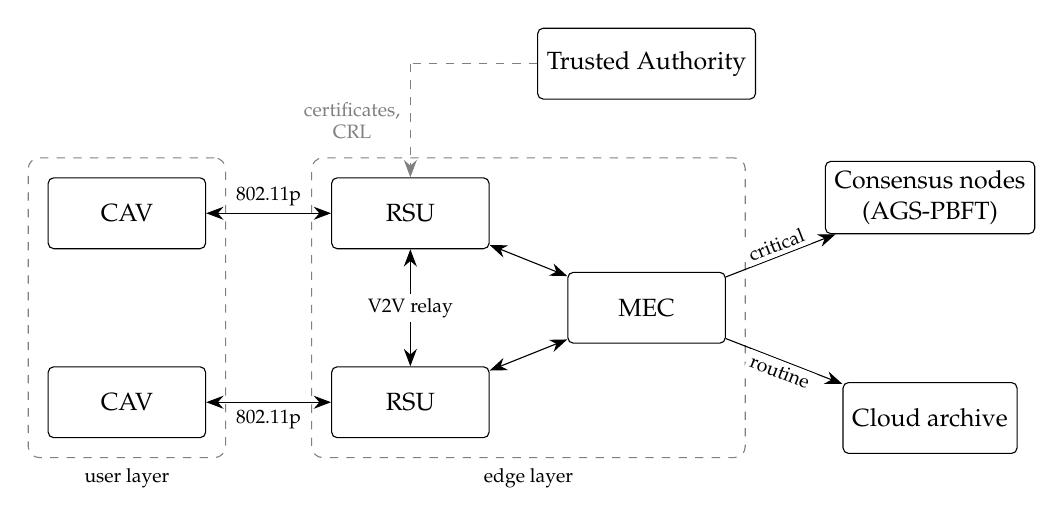
\begin{tikzpicture}[
  box/.style={draw, rounded corners=2pt, minimum height=9mm, minimum width=20mm, align=center, font=\small, fill=white},
  lab/.style={font=\scriptsize, align=center, fill=white, inner sep=1.5pt},
  layer/.style={draw, dashed, rounded corners=4pt, inner sep=7pt, gray},
  >={Stealth[length=2.2mm]}]
\node[box] (cav1) at (0,1.2) {CAV};
\node[box] (cav2) at (0,-1.2) {CAV};
\node[box] (rsu1) at (3.6,1.2) {RSU};
\node[box] (rsu2) at (3.6,-1.2) {RSU};
\node[box] (mec) at (6.6,0) {MEC};
\node[box] (cons) at (10.2,1.4) {Consensus nodes\\(AGS-PBFT)};
\node[box] (cloud) at (10.2,-1.4) {Cloud archive};
\node[box] (ta) at (6.6,3.1) {Trusted Authority};
\node[layer, fit=(cav1)(cav2), label={[font=\scriptsize]below:user layer}] {};
\node[layer, fit=(rsu1)(rsu2)(mec), label={[font=\scriptsize]below:edge layer}] {};
\draw[<->] (cav1) -- node[lab, above=1pt]{802.11p} (rsu1);
\draw[<->] (cav2) -- node[lab, below=1pt]{802.11p} (rsu2);
\draw[<->] (rsu1) -- node[lab]{V2V relay} (rsu2);
\draw[<->] (rsu1) -- (mec);
\draw[<->] (rsu2) -- (mec);
\draw[->] (mec) -- node[lab, above, sloped]{critical} (cons);
\draw[->] (mec) -- node[lab, below, sloped]{routine} (cloud);
\draw[dashed, gray] (ta.west) -- (3.6,3.1);
\draw[->, dashed, gray] (3.6,3.1) -- node[lab, left=2pt, text=gray]{certificates,\\CRL} (rsu1.north);
\end{tikzpicture}
\caption{Entities and links. The MEC sends alerts back through the RSUs before it submits a critical event to consensus.}
\label{fig:arch}
\end{figure}

\begin{description}
\item[Trusted Authority (TA).] Generates the root key pair, certifies the
public keys of all entities, keeps the registry database and signs the
certificate revocation list (CRL).
\item[CAV.] A vehicle. It holds its own ML-DSA key pair and certificate,
opens a session with the nearest RSU, sends beacons at 10\,Hz and reports
events.
\item[RSU.] Terminates vehicle sessions, relays V2V messages to neighbouring
RSUs, and forwards events to the MEC over the wired backhaul.
\item[MEC.] The edge server. It routes events by criticality: a critical
event is first turned into an alert sent to every RSU (and so to every
vehicle), \emph{then} submitted to consensus; routine data goes to the cloud.
\item[Consensus nodes.] Eight validators running AGS-PBFT. Each committed
block carries the event, the agreed validation result, a commit certificate,
the score table and the consensus membership.
\item[Cloud.] An archive for routine data.
\end{description}

\section{Threat model}

The adversary controls the radio: it can record, drop, delay, replay, modify
and inject any frame, and it can run its own transmitters. It may obtain copies
of any certificate (they are public), run a rogue certificate authority, and
hold credentials that the TA has since revoked. Up to $f$ consensus nodes may
be Byzantine (arbitrary behaviour, including colluding on a wrong result), and
a leader may crash. In the long term the adversary has a quantum computer and
replays recorded traffic to it. The TA's private key and the private keys of
honest entities are not compromised.

\section{Registration and PKI}

\begin{enumerate}
\item The entity generates its own ML-DSA key pair. The TA never sees a
private key (this removes the key escrow of defect D4).
\item The entity sends $\{id, role, pk, alg\}$ and a proof of possession: a
signature over the request with the new private key. Without it an attacker
could have someone else's public key certified under its own name.
\item The TA checks the identity against its roster (the identities vetted out
of band, such as manufacturer records and the RSU deployment list), the
algorithm, the key length and the proof, and returns
\[ Cert = \mathsf{Sign}(sk_{TA},\ \{id, role, pk, alg, serial, nb, na\}). \]
\item The entity verifies the certificate with $pk_{TA}$ before using it.
\end{enumerate}

The certificate binds the \emph{role}, so a vehicle cannot present itself as
an RSU, and a validity period and serial number, so it can expire and be
revoked. An ML-DSA-65 certificate is \V{deck-cert} bytes. Revocation is a
TA-signed CRL holding a version number, an issue time and the revoked serial
numbers; nodes accept only a
newer, validly signed CRL and close any open session with a revoked peer.

\section{Handshake}
\label{sec:handshake}

Figure~\ref{fig:hs} shows the four-flight handshake between a client
(initiator, usually a vehicle) and a server (responder, usually an RSU).

\begin{figure}[h]
\centering
\begin{adjustbox}{max width=\linewidth}
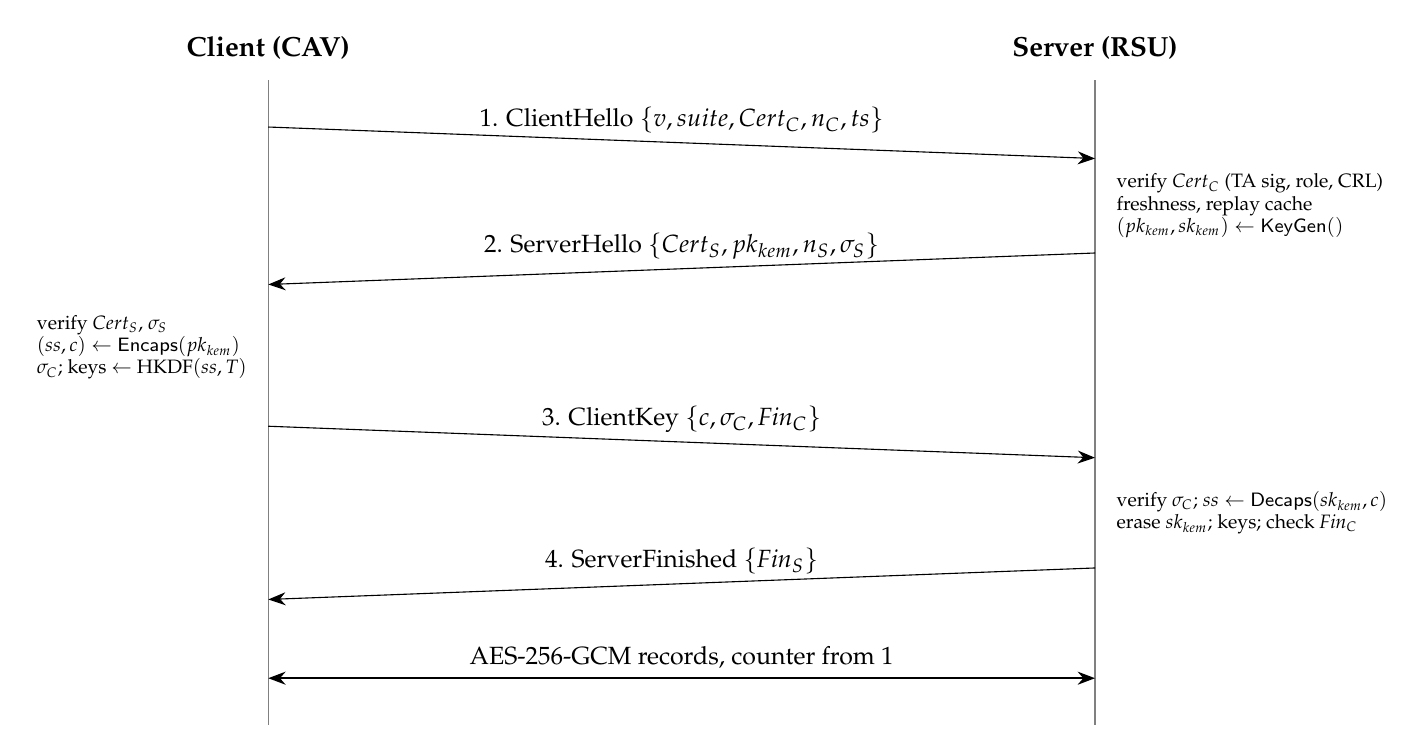
\begin{tikzpicture}[font=\small, >={Stealth[length=2.2mm]}]
\def\L{0} \def\R{10.5}
\node[font=\bfseries] at (\L,0.4) {Client (CAV)};
\node[font=\bfseries] at (\R,0.4) {Server (RSU)};
\draw[gray] (\L,0) -- (\L,-8.2); \draw[gray] (\R,0) -- (\R,-8.2);
\draw[->] (\L,-0.6) -- node[above]{1. ClientHello $\{v, suite, Cert_C, n_C, ts\}$} (\R,-1.0);
\node[align=left, font=\scriptsize, anchor=west] at (\R+0.15,-1.6)
  {verify $Cert_C$ (TA sig, role, CRL)\\freshness, replay cache\\$(pk_{kem}, sk_{kem}) \leftarrow \mathsf{KeyGen}()$};
\draw[<-] (\L,-2.6) -- node[above]{2. ServerHello $\{Cert_S, pk_{kem}, n_S, \sigma_S\}$} (\R,-2.2);
\node[align=left, font=\scriptsize, anchor=east] at (\L-0.15,-3.4)
  {verify $Cert_S$, $\sigma_S$\\$(ss, c) \leftarrow \mathsf{Encaps}(pk_{kem})$\\$\sigma_C$; keys $\leftarrow$ HKDF$(ss, T)$};
\draw[->] (\L,-4.4) -- node[above]{3. ClientKey $\{c, \sigma_C, \mathit{Fin}_C\}$} (\R,-4.8);
\node[align=left, font=\scriptsize, anchor=west] at (\R+0.15,-5.5)
  {verify $\sigma_C$; $ss \leftarrow \mathsf{Decaps}(sk_{kem}, c)$\\erase $sk_{kem}$; keys; check $\mathit{Fin}_C$};
\draw[<-] (\L,-6.6) -- node[above]{4. ServerFinished $\{\mathit{Fin}_S\}$} (\R,-6.2);
\draw[<->, thick] (\L,-7.6) -- node[above]{AES-256-GCM records, counter from 1} (\R,-7.6);
\end{tikzpicture}
\end{adjustbox}
\caption{The mutually authenticated handshake. $T$ is the transcript of all four flights.}
\label{fig:hs}
\end{figure}

\begin{align*}
\sigma_S &= \mathsf{Sign}(sk_S,\ \text{``sh''} \parallel H(CH, SH_{body})) \\
\sigma_C &= \mathsf{Sign}(sk_C,\ \text{``ck''} \parallel H(CH \parallel SH \parallel CK_{body})) \\
T_{hash} &= H(CH \parallel SH \parallel CK_{body} \parallel \sigma_C) \\
(k_{c2s}, v_{c2s}, k_{s2c}, v_{s2c}) &= \mathrm{HKDF}(ss, T_{hash}) \\
\mathit{Fin}_C &= \mathrm{AES\text{-}GCM}(k_{c2s}, v_{c2s} \oplus 0, H(\text{``client\_finished''}, T_{hash}))
\end{align*}

Design properties:
\begin{itemize}
\item \textbf{Forward secrecy.} The server's KEM key pair is ephemeral and
erased after decapsulation, so a later compromise of long-term signing keys
does not reveal past session keys.
\item \textbf{Mutual authentication.} $\sigma_S$ binds the server's identity
to the client's fresh nonce and to $pk_{kem}$; $\sigma_C$ binds the client's
identity to the whole transcript including the ciphertext $c$.
\item \textbf{Key confirmation.} Because ML-KEM rejects implicitly, a
tampered $c$ silently produces a different key. The Finished messages detect
it: each side proves it derived the same keys.
\item \textbf{Downgrade protection.} The suite is in the ClientHello, must
match exactly, and is covered by both signatures.
\item \textbf{Uniform abort.} Every failed check raises the same error with no
detail, so a probing attacker cannot tell which check failed.
\item \textbf{Sans-IO.} The handshake state machines consume and return bytes
and never touch a socket, so the same code runs over TCP, in memory for tests
and benchmarks, and supplies exact message sizes to ns-3.
\end{itemize}

\section{Certificate caching}
\label{sec:cache}

With ML-DSA-65 each certificate is \V{deck-cert} bytes, and the full handshake
carries two of them: about half of its \V{deck-hs-bytes} bytes. Peers usually
hold these certificates already. RSU certificates are few and long-lived, so
they can be distributed to vehicles in advance with the CRL. A vehicle's
certificate can be kept, after its first handshake, in an edge directory at the
MEC that every RSU reaches over the wired backhaul.

When a peer is known to hold a certificate, the handshake sends a 32-byte
reference $\mathit{cref} = H(\text{``qrcav-cert''}, Cert)$ instead, in the
spirit of TLS cached information~\cite{rfc7924}:

\begin{enumerate}
\item ClientHello carries $\mathit{cref}_C$ instead of $Cert_C$ once the
vehicle's certificate is in the directory, and $known = H(Cert_S)$ when the
vehicle holds the RSU's certificate.
\item If $known$ matches, ServerHello carries $\mathit{cref}_S$ instead of
$Cert_S$.
\item If the RSU cannot resolve $\mathit{cref}_C$ (locally or from the
directory) it answers \emph{HelloRetry} $\{n_C\}$, and the client resends its
ClientHello with the full certificate and a new nonce.
\end{enumerate}

The security argument:
\begin{itemize}
\item \textbf{Checks are not cached.} A cached certificate is verified in full
on every handshake (TA signature, validity, role, expected identity, current
CRL), so revocation still takes effect at the next CRL refresh.
\item \textbf{The reference is bound by both signatures.} $\mathit{cref}$ is
a collision-resistant hash of the exact certificate bytes and lies inside the
messages that $\sigma_C$ and $\sigma_S$ cover. Claiming another vehicle's
cached certificate fails $\sigma_C$; replacing the server's reference fails
$\sigma_S$.
\item \textbf{The directory is not trusted.} A fetched certificate must hash
to the requested reference and is verified against $pk_{TA}$.
\item \textbf{The cache cannot be filled by strangers.} A server caches a
client certificate only after a handshake with its owner has completed, and
the cache is a bounded LRU.
\item \textbf{HelloRetry is unauthenticated, and that is acceptable.} It must
echo the client's nonce and is honoured once per handshake. Forging it only
forces the full-certificate path, the same property as TLS~1.3's
HelloRetryRequest~\cite{tls13}.
\end{itemize}

For DECK the handshake shrinks from \V{deck-hs-bytes} to
\V{deck-cached-bytes} bytes (\V{deck-cache-saving}\,\% smaller) and from
\V{deck-hs-frames} to \V{deck-cached-frames} radio frames. The cached
ClientHello is \V{deck-ch-cached} bytes, one frame.

\section{Record layer}

\begin{align*}
record &= ctr\ (8\,\mathrm{B}) \parallel \mathrm{AES\text{-}256\text{-}GCM}(k_{dir},\ nonce,\ pt,\ aad = dir \parallel ctr) \\
nonce &= v_{dir} \oplus (0^{32} \parallel \mathrm{be64}(ctr))
\end{align*}

Counter 0 is reserved for the Finished message and application data starts at
1, so no (key, nonce) pair is ever reused. A 64-record sliding window accepts
reordered records once and rejects replays; it is checked \emph{before}
decryption, so a replay flood costs a lookup rather than an AES operation. A
session refuses to send more than $2^{32}$ records.

\section{Defects found and corrected}
\label{sec:defects}

\subsection{In the base paper}

\begin{table}[h]
\centering
\caption{Defects in the base paper and their corrections}
\label{tab:defects}
\begin{tabular}{@{}p{0.6cm}p{6.2cm}p{6.8cm}@{}}
\toprule
& Defect & Correction \\
\midrule
D1 & Consensus messages are signed and verified ``using Kyber'', a KEM with no signing operation. & ML-DSA signatures on every consensus message. \\
D2 & The encapsulation listing defines $k_i$ in terms of itself, and decapsulation uses $k_i$, which the receiver does not have. & The standard \textsf{Encaps}/\textsf{Decaps} interface. \\
D3 & The session key is $H(k_i \parallel k'_j)$, a value hashed with itself, since a correct KEM gives $k_i = k'_j$. & HKDF over the shared secret and the hash of the whole transcript. \\
D4 & The TA generates entities' private keys (key escrow) although the paper claims ``no key escrow''. & Entities generate their own keys; the TA certifies public keys only, with proof of possession. \\
D5 & Hyperledger Fabric 2.2 orders with Raft and cannot host a PBFT-family protocol. & A ledger implemented directly, driven by AGS-PBFT. \\
\bottomrule
\end{tabular}
\end{table}

\subsection{In our Review 1 design}

\begin{table}[h]
\centering
\caption{Corrections to the Review 1 handshake design}
\label{tab:fixes}
\begin{tabular}{@{}p{0.6cm}p{6.2cm}p{6.8cm}@{}}
\toprule
& Review 1 & Now, and why \\
\midrule
F1 & The server signs $T \parallel pk_{kem}$, but nothing initialises $T$. & A ClientHello with a fresh nonce and timestamp opens $T$, so a recorded ServerHello cannot be replayed. \\
F2 & Only the server signs. & The client signs the transcript. Otherwise anyone holding a copy of a vehicle's (public) certificate can open a session as that vehicle. \\
F3 & Finished uses counter 0; where data starts is unspecified. & Data starts at counter 1: no GCM nonce reuse. \\
F4 & Key generation shown as $sk_{kem} \leftarrow (s, e, pk_{kem})$. & \textsf{KeyGen()}; FIPS 203's $dk$ is $(s, ek, H(ek), z)$. \\
F5 & The certificate signs only $ID \parallel pk$. & Role, serial and validity are bound too. \\
F6 & No downgrade protection. & Suite in the ClientHello, matched exactly, signed. \\
F7 & Abort reasons unspecified. & One uniform error. \\
\bottomrule
\end{tabular}
\end{table}

\section{Edge routing}

Each event carries a criticality level set by the reporting vehicle, and the
MEC routes on it. A critical event (collision ahead, pedestrian on the road,
ice) is broadcast as an alert to every RSU, which re-encrypts it
for each vehicle's session, and only then submitted to consensus for the
ledger. A routine event (a pothole report, road condition) goes to the cloud
archive. Safety warnings therefore never wait for a consensus round.

\section{AGS-PBFT}

\subsection{Normal case}

\begin{enumerate}
\item The MEC sends a signed REQUEST to the leader, $R[v \bmod |R|]$, where
$R$ is the sorted consensus set.
\item The leader sends a signed PRE-PREPARE to the consensus set and to the
candidates.
\item Consensus nodes broadcast PREPARE. On $2f+1$ matching prepares each node
\emph{validates} the event (fields present, reporter's TA certificate valid,
event not already recorded) and sends its result in a RESPONSE to the leader.
Candidates send a SHADOW-RESPONSE that is scored but not counted towards the
quorum.
\item On $2f+1$ matching responses the leader builds a block containing the
request, the agreed result, the signed responses as a commit certificate, the
updated scores and the membership, signs it, sends COMMIT to every node and
REPLY to the MEC.
\item Every node re-verifies the block (hash link, leader signature, commit
certificate, recomputed scores and membership) before appending it.
\end{enumerate}

\subsection{Scores and regrouping}

A node gains $+1$ if its result matches the committed one and loses $5$ if it
differs. Every \emph{regroup interval} (50 blocks in the paper), nodes compute
$\mu$ and $\sigma$ over all scores; consensus nodes below $\mu - \sigma$ are
demoted and candidates above $\mu + \sigma$ promoted, and the set is resized
to $3f+1$. Because scores and membership are written into each block and
re-derived by every node, all nodes agree on the consensus set without extra
messages.

\subsection{Decisions where the paper is undefined}

\begin{table}[h]
\centering
\caption{Design decisions for AGS-PBFT}
\label{tab:dd}
\begin{tabular}{@{}p{0.6cm}p{6.2cm}p{6.8cm}@{}}
\toprule
& Gap in the paper & Decision \\
\midrule
D6 & All nodes start at 100, so at the first regroup $\sigma = 0$ and $\mu - \sigma = \mu + \sigma$: every node is both above and below threshold. & Skip regrouping while $\sigma = 0$. \\
D7 & Candidates never take part, so they can never gain score or be promoted. & Candidates validate as shadows and are scored. Absent nodes score 0, not $-5$, so a Byzantine leader cannot punish honest nodes by omitting their responses. \\
D8 & ``Group size is adjusted based on network activity'' is not specified. & Request rate $r$ over the interval, from request timestamps so every node computes the same value: $f$ falls linearly from $f_{max}$ at $r \le 2$/s to 1 at $r \ge 20$/s. \\
D9 & $2f+1$ prepares are required, but the leader sends none, so the quorum is unreachable with $f$ faulty backups. & The leader also sends a PREPARE for its own proposal. \\
\bottomrule
\end{tabular}
\end{table}

\subsection{View change}

A consensus node that has seen a request but not its commit within a timeout
broadcasts VIEW-CHANGE$\{v+1, h, head, P\}$, where $P$ holds its prepared
certificates above its ledger height $h$. On $2f+1$ view changes the new
leader computes the set $O$ of requests to re-issue (the highest-view prepared
request for each sequence number, or a no-op for a gap) and sends
NEW-VIEW$\{v+1, V, O\}$. Replicas verify the signatures, recompute $O$, and on
a match enter the new view. The timeout doubles after each failed view.
Messages for a future view are buffered, because a pre-prepare can overtake
the NEW-VIEW that precedes it.

\section{Ledger}

A block is $(B\_ID, Pr\_B\_Hash, T\_Block)$ as in the paper, plus view,
sequence number, signed request, agreed result, commit certificate, score
table, membership, leader identity and leader signature. Any party holding
$pk_{TA}$ can replay a ledger from genesis and check every hash link,
signature, certificate, score and membership change.

\chapter{Implementation}
\label{ch:impl}

\section{Software structure}

The system is a Python package, \code{qrcav}, with a strict layering: lower
layers never import upper ones, and the protocol code performs no I/O.

\begin{table}[h]
\centering
\caption{Package structure}
\label{tab:modules}
\begin{tabular}{@{}p{4.9cm}p{9.1cm}@{}}
\toprule
Module & Responsibility \\
\midrule
\code{crypto/suites.py} & ML-KEM and ML-DSA behind one interface (OpenSSL); ECDH/ECDSA baseline \\
\code{crypto/kdf.py} & SHAKE-256 hash, HKDF-SHA3-256, session key derivation \\
\code{crypto/records.py} & AES-256-GCM records, counters, replay window \\
\code{codec.py} & canonical compact binary encoding (signatures need identical bytes on both sides) \\
\code{pki.py} & Trusted Authority, certificates, CRL, registry database, identities \\
\code{handshake.py} & the four-flight handshake as sans-IO state machines \\
\code{certcache.py} & certificate references and the bounded LRU cache \\
\code{consensus/agspbft.py} & AGS-PBFT and PBFT replica: normal case, scoring, regrouping, view change \\
\code{consensus/sim.py} & discrete-event harness running real replicas with real signatures \\
\code{ledger.py} & hash-linked, certified blocks; full-chain verification \\
\code{net/secure.py} & secure channels over TCP with length framing \\
\code{nodes/} & one process per entity: TA, CAV, RSU, MEC, consensus node, cloud \\
\code{sim/} & ns-3 scenario (C++), its Python driver, measurement profiles \\
\code{eval/} & benchmarks, attack harness, consensus experiments, ns-3 sweeps, figures, replay viewer \\
\bottomrule
\end{tabular}
\end{table}

\section{Cryptographic suites}

A \emph{suite} pairs a KEM with a signature scheme. Five are implemented:
\textbf{DECK} (ML-KEM-1024 + ML-DSA-65, the pairing in our Review~1 design and
in~\cite{olushola}), \textbf{L1} (512/44), \textbf{L3} (768/65), \textbf{L5}
(1024/87), and \textbf{CLASSIC} (ECDH P-256 + ECDSA P-256, as in IEEE~1609.2).
DECK pairs a category-5 KEM with a category-3 signature, so its overall
strength is category~3, the same as L3.

ECDH is wrapped as a KEM with the DHKEM construction of RFC~9180~\cite{hpke}:
\textsf{Encaps} generates an ephemeral key pair, computes the Diffie--Hellman
value with the receiver's public key, hashes it together with both public
keys, and sends the ephemeral public key as the ``ciphertext''. The classical
baseline therefore runs through exactly the same handshake code as the
post-quantum suites, which makes the comparison like-for-like.

All algorithms come from the \code{cryptography} library (version 47 or
later), which bundles OpenSSL~3.5 with native, constant-time ML-KEM and
ML-DSA, as a deployment would use. One exception: the library exposes
ML-KEM-768 and ML-KEM-1024 but not ML-KEM-512, so the L1 suite takes its KEM
from \code{kyber-py}, a pure-Python implementation of FIPS~203. It produces
the same sizes and encodings, but it is slower and, as its authors state, not
constant-time, which is why L1's handshake is the slowest in
Section~\ref{ch:results}.

\section{Distributed system}

Every entity is a separate operating-system process started from one
configuration file. A run of the demonstration scenario starts 19 processes:
the TA, the cloud, one MEC, eight consensus nodes, three RSUs and five
vehicles. Transport is TCP with a 4-byte length prefix per frame; the four
handshake flights are frames, and afterwards every frame is one AES-GCM
record. Registration and CRL retrieval use plain TCP, which is safe because
certificates and CRLs are TA-signed and verified on receipt. Each process
writes structured JSON logs, from which an end-to-end report is produced.

The configuration injects faults: a consensus node can return wrong results
(\code{wrong\_result}) or stay silent, a node can crash at a given time, the
TA can revoke an entity, and vehicles follow a script of events, V2V messages,
handovers and reconnections.

\section{ns-3 simulation}

\subsection{Method}

ns-3 3.44~\cite{ns3} simulates the radio, MAC, backhaul and mobility. The
scenario is written in C++ and compiled at run time through the ns-3 Python
bindings. ns-3 does not execute the Python cryptography, which would mix
wall-clock and simulated time. Instead the real protocol code is run first to
produce a \emph{measurement profile}: the exact byte length of every message
(the four handshake flights, cached flights, AEAD and signed beacons, events,
alerts) and empirical samples of the processing time at each handshake stage,
per beacon, and for a consensus commit. The simulation draws from these
samples whenever a node processes a message, and each node has a
single-server CPU queue.

\begin{table}[h]
\centering
\caption{ns-3 scenario}
\label{tab:ns3}
\begin{tabular}{@{}p{4.2cm}p{9.8cm}@{}}
\toprule
Parameter & Value \\
\midrule
Radio & IEEE 802.11p, channel 172 (5.86\,GHz), 10\,MHz, 6\,Mb/s, 23\,dBm \\
Propagation & log-distance ($n = 2.2$) + Nakagami fading, $m = 3 / 1.5 / 1$ below 50 / 150 / beyond~\cite{torrent} \\
Detection, CCA & $-85$\,dBm (the 10\,MHz value) \\
Area & 1.5\,km $\times$ 1.5\,km Manhattan grid, 250\,m blocks \\
RSUs & at intersections every 500\,m: 9 RSUs, wired to one MEC (1\,Gb/s, 2\,ms) \\
Vehicles & 50--200; 8--17\,m/s; straight 50\,\%, left or right 25\,\% each at intersections \\
Beacons & 10\,Hz link-layer broadcast (no ACK, no retry) \\
Fragmentation & 1,400-byte chunks; reassembly at the receiver \\
Handshake & 200\,ms timeout, 3 retries; NACK for missing ServerHello chunks \\
Association & start once $\ge 6$ of 10 announcements per second are heard; handover to an RSU heard $\ge 4$ per second better \\
EDCA & beacons, events, alerts as AC\_VO; handshake flights as AC\_BE \\
Backoff & after a failed handshake wait $U(0.5, 1) \times 2^k$\,s \\
Run & 30\,s simulated, first 5\,s excluded; 3 seeds \\
\bottomrule
\end{tabular}
\end{table}

\subsection{Simulator pitfalls found and corrected}

Five ns-3 defaults distorted results by an order of magnitude before they
were corrected, and they belong in any reproduction of this work:
\begin{enumerate}
\item \textbf{ARP.} The ARP cache queues only three packets per unresolved
address, so most fragments of a first ServerHello were silently dropped.
802.11p safety messaging has no ARP, so neighbour caches are pre-populated.
\item \textbf{Preamble detection.} ns-3 defaults to the 20\,MHz value of
$-82$\,dBm; 802.11p's 10\,MHz channel uses $-85$\,dBm. The wrong value cut
coverage from 99\,\% to about 80\,\%.
\item \textbf{Unicast beacons} suffered up to 7 MAC retries each; real beacons
are broadcasts.
\item \textbf{Whole-flight retransmission} after one lost fragment caused a
retransmission storm; it was replaced with selective retransmission.
\item \textbf{First-contact association.} Starting a 17-frame handshake on the
first announcement heard, usually at the edge of coverage, gave 5\,\%
success; association is now gated on link quality.
\end{enumerate}

\subsection{Certificate caching in the simulation}

Mode 1 models the deployment of Section~\ref{sec:cache}: RSU certificates are
pre-distributed, so every ServerHello carries a reference; after its first
session a vehicle sends a reference too, and an RSU that has not seen the
vehicle resolves it from the MEC directory at the cost of one backhaul round
trip (no airtime). Mode 2, used as an upper bound, starts with all caches warm.

\subsection{Replay viewer}

For demonstration, the simulation can record an event trace (handshake
start, session up, failure, link loss, handover, event, alert) and the
channel airtime in 0.5\,s buckets. A script runs the same scenario (same
mobility and seed) for the classical suite, DECK and DECK with caching, and
writes a self-contained web page that replays the three runs on the city grid
(Figure~\ref{fig:viewer}).

\section{Evaluation harness}

\begin{itemize}
\item \textbf{Primitives}: 200 timed runs per operation, after warm-up runs
are discarded.
\item \textbf{Handshakes}: 100 complete handshakes per suite in memory,
recording each stage's processing time and every flight's size, with and
without caching.
\item \textbf{Beacon budget}: per-beacon cryptography plus airtime for AEAD
records and for signed broadcasts.
\item \textbf{Attacks}: \V{attacks-total} attacks run against the real
implementation; an attack counts as rejected only if the protocol aborts or
drops the message.
\item \textbf{Consensus}: real replicas with real ML-DSA signatures in a
discrete-event loop, for 8--24 nodes, AGS-PBFT with and without shadow
validation against PBFT; fault tolerance; view change; score dynamics.
\item \textbf{ns-3 sweeps}: five suites and DECK with caching at 50--200
vehicles over three seeds, plus single-seed variants.
\end{itemize}
Timing measurements were taken with the machine otherwise idle, because
benchmarks run alongside ns-3 inflated latencies.

\section{Testing}

55 automated tests (\code{pytest}) cover the codec, FIPS key and signature sizes, key derivation (output lengths and transcript binding), record
counters and replay window, ML-KEM-512 sizes, registration (proof of
possession, roster, duplicate keys), handshakes for all suites, role checks,
certificate caching (savings, fallback, revocation, substituted references,
forged HelloRetry), AGS-PBFT (normal case, scoring, regrouping, view change,
Byzantine nodes, determinism) and one complete multi-process run of the
distributed system.

\section{Bugs found by our own verification}

\begin{enumerate}
\item \textbf{Consensus stalled about once in 14 runs.} Nodes checked whether
the reporting vehicle was registered against the registry copy each had
fetched at start-up; a node that started before the vehicle enrolled
disagreed with the rest, and with one Byzantine node in a set of four no
result reached $2f+1$. Found by tracing every message of a failing run, fixed
by carrying the reporter's TA-signed certificate in the request so validation
is a pure function of the request, and verified with 0 failures in 25 runs.
\item \textbf{Sequence-number reuse after a view change}: the new leader
re-issued prepared requests and then reused their numbers.
\item \textbf{PRE-PREPAREs overtaking NEW-VIEW} were dropped as wrong-view;
they are now buffered and replayed.
\item \textbf{Measurement contention}: timings taken while ns-3 used both
cores were inflated and were re-measured.
\end{enumerate}

\chapter{Results and Discussion}
\label{ch:results}

All numbers in this chapter are generated from the CSV files the evaluation
scripts write (\code{results/}), and all timings were measured on a 2-core
cloud virtual machine with the CPU otherwise idle. Absolute timings on other
hardware differ; the comparisons between suites do not.

\section{Cryptographic cost}

\subsection{Primitives}

\begin{table}[h]
\centering
\caption{Primitive operations (ms)}
\label{tab:prim}
\small
\begin{adjustbox}{max width=\linewidth}
\begin{tabular}{lrrrrrr}
\toprule
Suite & KEM keygen & encaps & decaps & sign & sign p99 & verify \\
\midrule
Classical & 0.024 & 0.12 & 0.091 & 0.031 & 0.072 & 0.12 \\
L1 (KEM in kyber-py) & 1.80 & 2.70 & 3.63 & 1.27 & 3.32 & 0.16 \\
L3 & 0.14 & 0.052 & 0.041 & 1.30 & 4.60 & 0.23 \\
DECK & 0.23 & 0.067 & 0.052 & 1.28 & 4.38 & 0.23 \\
L5 & 0.20 & 0.067 & 0.052 & 1.48 & 5.19 & 0.42 \\
\bottomrule
\end{tabular}
\end{adjustbox}
\par\smallskip{\footnotesize Mean of 200 runs after warm-up, in ms. All operations use OpenSSL through the \texttt{cryptography} library, except L1's ML-KEM-512, which that library does not expose; it comes from \texttt{kyber-py} (pure Python).}

\end{table}

Table~\ref{tab:prim} gives two findings. First, \textbf{signing is the only
expensive post-quantum operation, and its variance is intrinsic}: ML-DSA's
rejection sampling repeats until a candidate passes, so the 99th percentile
is several times the mean in both backends, while verification is
deterministic and fast. Second, \textbf{the implementation matters more than
the algorithm}: the same ML-DSA-65 signs in \V{deck-sign-native}\,ms natively
and \V{deck-sign-pure}\,ms in pure Python, a factor of about \V{sign-speedup}.
Our Review~1 conclusion, that signing might not fit the 100\,ms budget, was a
property of the pure-Python library, not of ML-DSA.

\subsection{Handshake size and compute}

\begin{table}[h]
\centering
\caption{Key, signature, certificate and handshake sizes (bytes), with and without certificate caching}
\label{tab:sizes}
\scriptsize
\setlength{\tabcolsep}{3.2pt}
\begin{adjustbox}{max width=\linewidth}
\begin{tabular}{lllrrrrrrrrr}
\toprule
Suite & KEM & Signature & pk$_\text{KEM}$ & sig & cert & bytes & frames & air (ms) & cached & frames & saving \\
\midrule
Classical & ECDH-P256 & ECDSA-P256 & 65 & 70 & 229 & 1{,}043 & 4 & 2.05 & 691 & 4 & 33.7\,\% \\
L1 & ML-KEM-512 & ML-DSA-44 & 800 & 2{,}420 & 3{,}826 & 14{,}373 & 13 & 21.3 & 6{,}825 & 8 & 52.5\,\% \\
L3 & ML-KEM-768 & ML-DSA-65 & 1{,}184 & 3{,}309 & 5{,}355 & 19{,}913 & 17 & 29.4 & 9{,}307 & 10 & 53.3\,\% \\
DECK & ML-KEM-1024 & ML-DSA-65 & 1{,}568 & 3{,}309 & 5{,}355 & 20{,}779 & 17 & 30.5 & 10{,}173 & 10 & 51.0\,\% \\
L5 & ML-KEM-1024 & ML-DSA-87 & 1{,}568 & 4{,}627 & 7{,}313 & 27{,}329 & 22 & 40.1 & 12{,}807 & 12 & 53.1\,\% \\
\bottomrule
\end{tabular}
\end{adjustbox}

\end{table}

\begin{figure}[h]
\centering
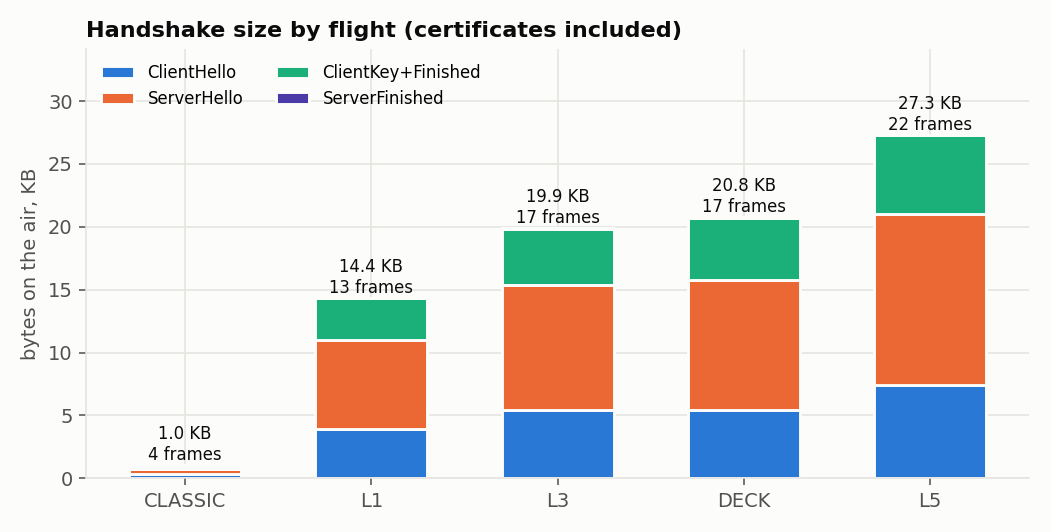
\includegraphics[width=0.9\textwidth]{fig2_handshake_size.png}
\caption{Handshake bytes by flight. The ServerHello carries the server's certificate, the ephemeral ML-KEM key and a signature.}
\label{fig:size}
\end{figure}

\begin{table}[h]
\centering
\caption{Compute time of one full handshake, both sides (ms)}
\label{tab:hstime}
\begin{adjustbox}{max width=\linewidth}
\begin{tabular}{lrr}
\toprule
Suite & mean & p95 \\
\midrule
Classical & 1.16 & 1.29 \\
L1 & 11.6 & 12.6 \\
L3 & 4.77 & 7.85 \\
DECK & 4.77 & 7.22 \\
L5 & 5.68 & 8.12 \\
\bottomrule
\end{tabular}
\end{adjustbox}
\par\smallskip{\footnotesize Compute time of one complete mutual handshake, both sides together, in ms (no network).}

\end{table}

A post-quantum handshake is \V{pq-size-ratio-lo}--\V{pq-size-ratio-hi} times
the size of the classical one (Table~\ref{tab:sizes},
Figure~\ref{fig:size}): \V{deck-hs-bytes} bytes in \V{deck-hs-frames} frames
for DECK against \V{classic-hs-bytes} bytes in \V{classic-hs-frames} frames,
or \V{deck-hs-air}\,ms of airtime against \V{classic-hs-air}\,ms. Certificates
are the largest single item, \V{deck-cert} bytes each. The Review~1 figure of
6,494 bytes left the certificates out.

Computation is small by comparison (Table~\ref{tab:hstime},
Figure~\ref{fig:compute}): about \V{deck-hs-ms}\,ms for a complete DECK
handshake natively against \V{classic-hs-ms}\,ms classically, but
\V{deck-hs-ms-pure}\,ms with the pure-Python library. With a native
implementation, \textbf{the cost of post-quantum V2X is bytes, not CPU time}.

\begin{figure}[h]
\centering
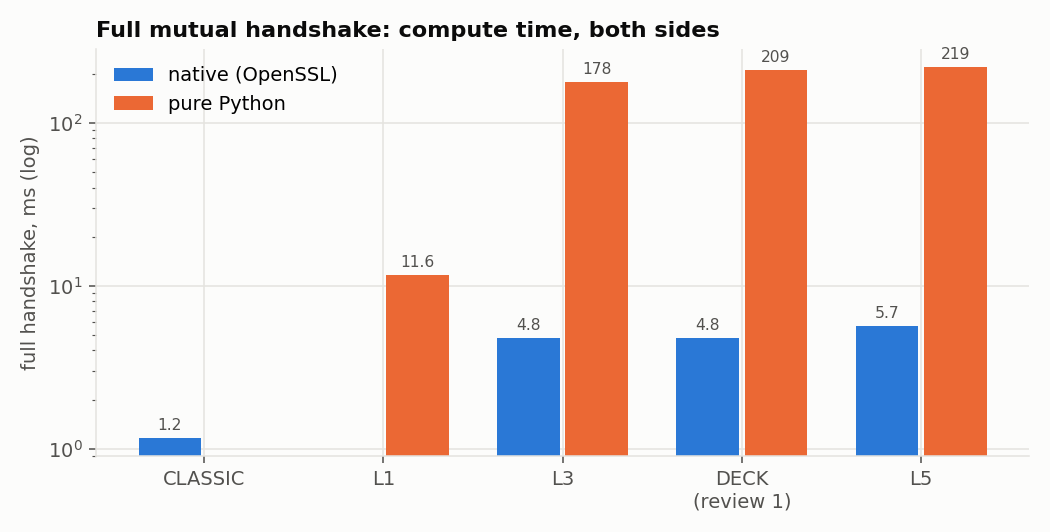
\includegraphics[width=0.85\textwidth]{fig1_handshake_compute.png}
\caption{Full handshake compute time, native and pure-Python backends (log scale).}
\label{fig:compute}
\end{figure}

\subsection{Per-beacon budget}

\begin{table}[h]
\centering
\caption{Per-beacon cost, p99 crypto plus airtime (ms)}
\label{tab:beacon}
\small
\begin{adjustbox}{max width=\linewidth}
\begin{tabular}{lrr}
\toprule
Suite & AEAD in a session & signed broadcast \\
\midrule
Classical & 0.40 (135 B) & 0.88 (234 B, 1 fr.) \\
L1 & 0.44 (135 B) & 5.55 (2{,}583 B, 2 fr.) \\
L3 & 0.41 (135 B) & 9.87 (3{,}472 B, 3 fr.) \\
DECK & 0.41 (135 B) & 9.51 (3{,}472 B, 3 fr.) \\
L5 & 0.47 (135 B) & 12.6 (4{,}790 B, 4 fr.) \\
\bottomrule
\end{tabular}
\end{adjustbox}
\par\smallskip{\footnotesize p99 of cryptographic processing plus 802.11p airtime per beacon, in ms, against the 100 ms beacon interval.}

\end{table}

The base paper folds the one-off handshake into its per-message latency.
Separated (Table~\ref{tab:beacon}, Figure~\ref{fig:beacon}), the per-beacon
cost inside a session is the same for every suite: a
\V{deck-beacon-aead-bytes}-byte AES-GCM record costing
\V{deck-beacon-aead}\,ms against a 100\,ms interval. Signing every beacon, as
IEEE~1609.2 does today, also fits natively (\V{deck-beacon-signed}\,ms for
DECK) but costs \V{deck-beacon-signed-bytes} bytes, \V{deck-beacon-signed-frames}
frames per beacon, and misses the deadline with the pure-Python library.

\begin{figure}[h]
\centering
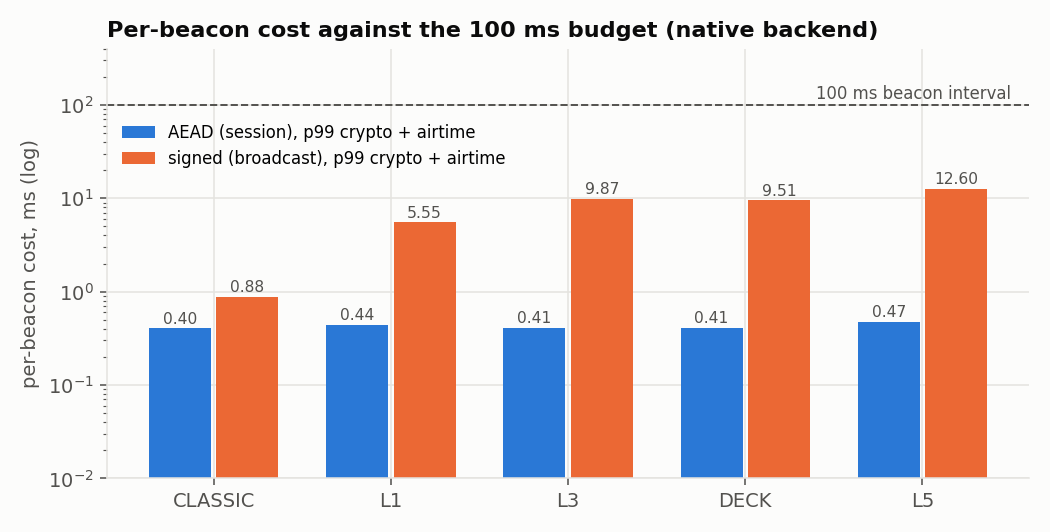
\includegraphics[width=0.85\textwidth]{fig3_beacon_budget.png}
\caption{Per-beacon cost against the 100\,ms beacon interval.}
\label{fig:beacon}
\end{figure}

\section{Distributed system}

One run of the demonstration scenario (19 processes over TCP on one machine)
established \V{net-handshakes} secure sessions (\V{net-hs-min}--\V{net-hs-max}
bytes each, depending on whether certificates travelled as references) and
rejected \V{net-rejected} handshakes from the revoked vehicle. Alerts reached
vehicles a median \V{net-alert-ms}\,ms after a critical event was reported,
while the event reached the ledger after a median \V{net-ledger-ms}\,ms: the
MEC sends the alert before it submits the event, so \textbf{the safety path
never waits for consensus}. The Byzantine node (wrong results) was demoted at
the first regroup and a candidate promoted; when the leader crashed, a view
change installed the next leader and later events committed; after the TA
revoked a vehicle, its session was closed and its reconnection rejected. All
eight ledger copies were consistent (the crashed leader's copy is a prefix
of the others) and verified from genesis.

\section{ns-3: 802.11p with mobility}

\subsection{Handshake success and latency}

\begin{table}[h]
\centering
\caption{Handshakes completed (\%) by vehicle density}
\label{tab:ns3success}
\small
\begin{adjustbox}{max width=\linewidth}
\begin{tabular}{lrrrrrr}
\toprule
Vehicles (/km$^2$) & Classical & L1 & L3 & DECK & L5 & DECK + cache \\
\midrule
50 (22) & 100 & 100 & 99 & 100 & 99 & 100 \\
100 (44) & 100 & 97 & 70 & 74 & 56 & 98 \\
150 (67) & 100 & 54 & 40 & 38 & 32 & 80 \\
200 (89) & 100 & 39 & 27 & 27 & 22 & 57 \\
\bottomrule
\end{tabular}
\end{adjustbox}
\par\smallskip{\footnotesize Handshakes completed, \%. Mean of 3 seeds; 1.5\,km $\times$ 1.5\,km Manhattan grid, 9 RSUs, IEEE 802.11p at 6\,Mb/s.}

\end{table}

\begin{table}[h]
\centering
\caption{Median handshake completion time (ms)}
\label{tab:ns3p50}
\small
\begin{adjustbox}{max width=\linewidth}
\begin{tabular}{lrrrrrr}
\toprule
Vehicles (/km$^2$) & Classical & L1 & L3 & DECK & L5 & DECK + cache \\
\midrule
50 (22) & 7 & 73 & 88 & 90 & 139 & 54 \\
100 (44) & 8 & 109 & 288 & 285 & 482 & 73 \\
150 (67) & 10 & 575 & 651 & 636 & 750 & 197 \\
200 (89) & 12 & 763 & 760 & 795 & 844 & 417 \\
\bottomrule
\end{tabular}
\end{adjustbox}
\par\smallskip{\footnotesize Median handshake completion time, ms. Mean of 3 seeds; 1.5\,km $\times$ 1.5\,km Manhattan grid, 9 RSUs, IEEE 802.11p at 6\,Mb/s.}

\end{table}

\begin{figure}[h]
\centering
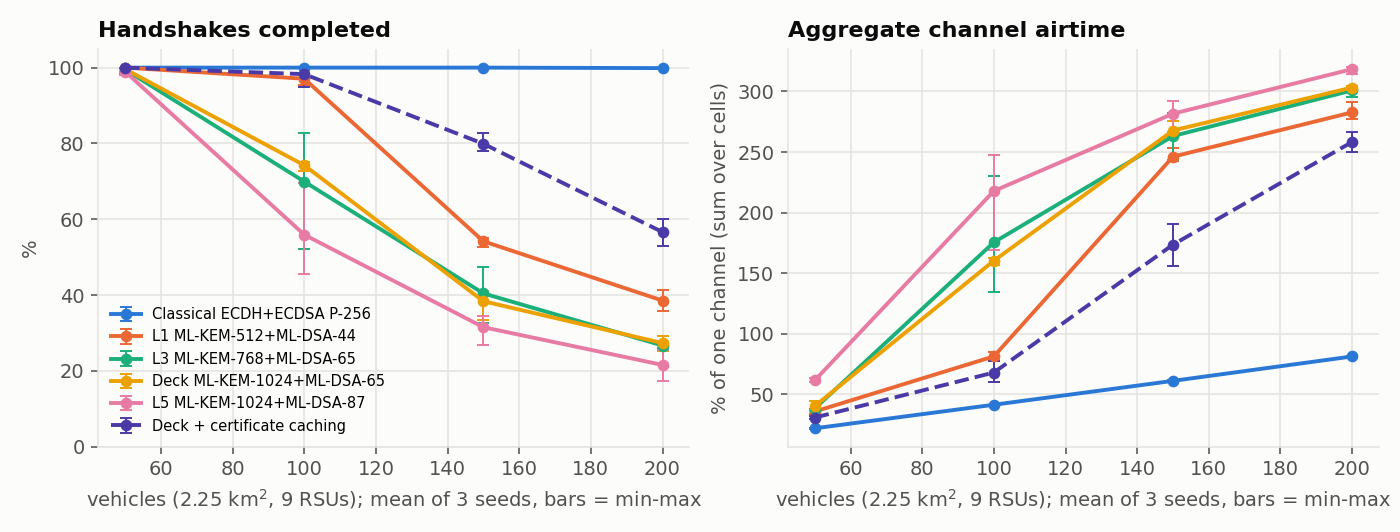
\includegraphics[width=\textwidth]{fig8_ns3_success_airtime.png}
\caption{Handshakes completed and aggregate channel airtime against density (mean of \V{ns3-seeds} seeds, bars show min--max).}
\label{fig:ns3success}
\end{figure}

\begin{figure}[h]
\centering
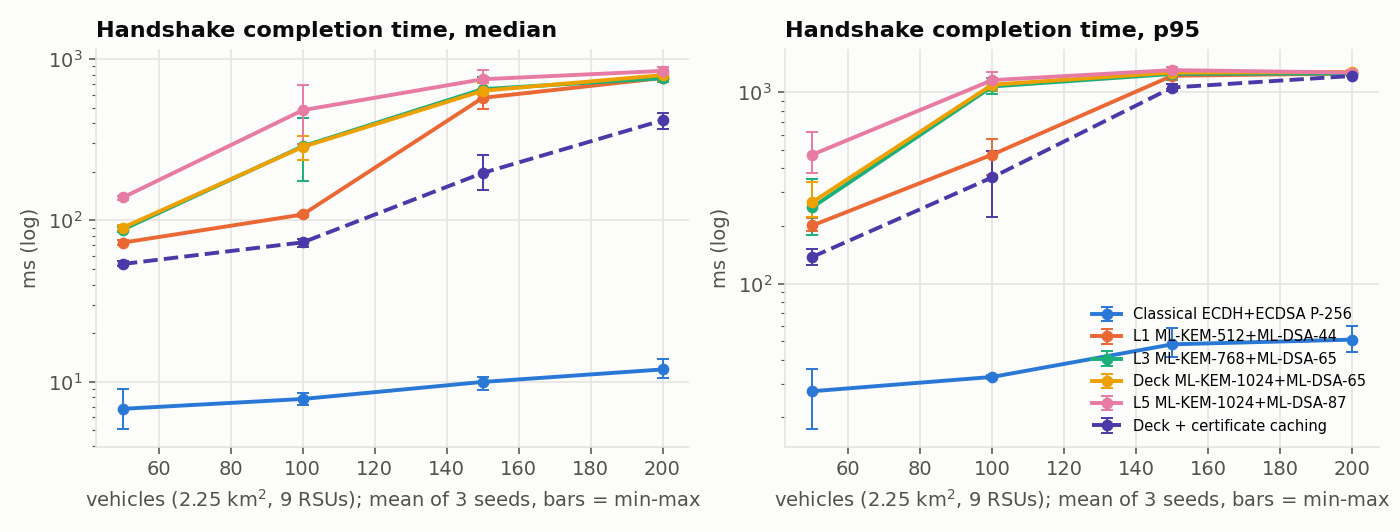
\includegraphics[width=\textwidth]{fig7_ns3_handshake_latency.png}
\caption{Handshake completion time, median and 95th percentile (log scale).}
\label{fig:ns3lat}
\end{figure}

Tables~\ref{tab:ns3success} and~\ref{tab:ns3p50} and
Figures~\ref{fig:ns3success}--\ref{fig:ns3lat} give the central result.
\textbf{The classical handshake completes \V{ns3-success-classic-200}\,\% of the
time even at 200 vehicles. Every post-quantum suite degrades with density},
roughly in order of handshake size: L1 (\V{l1-hs-kb}\,KB) holds up longest
and L5 (\V{l5-hs-kb}\,KB) fails first, while L3 and DECK, which differ by
less than 1\,KB, are within seed-to-seed variation of each other. At 100 vehicles (44 per
km$^2$) DECK completes \V{ns3-success-deck-100}\,\% of handshakes with a
median of \V{ns3-p50-deck-100}\,ms, against \V{ns3-p50-classic-100}\,ms
classically; at 200 vehicles it completes \V{ns3-success-deck-200}\,\%.
The cause is airtime: handshake fragments push the shared channel into
saturation, and losses then trigger retransmissions that add more load.

\subsection{Other measures}

\begin{table}[h]
\centering
\caption{Other measures at \V{ns3-mid} vehicles}
\label{tab:ns3mid}
\small
\begin{adjustbox}{max width=\linewidth}
\begin{tabular}{lrrr}
\toprule
Measure & Classical & DECK & DECK + cache \\
\midrule
Beacon slots with a session (\%) & 99.9 & 83.3 & 97.4 \\
Aggregate airtime (\% of one channel) & 41 & 160 & 68 \\
Handshake time, p95 (ms) & 33 & 1{,}094 & 359 \\
Event $\rightarrow$ alert at the reporter, median (ms) & 5.4 & 7.6 & 5.6 \\
Ledger commit after the event, median (ms) & 11.6 & 24.6 & 24.0 \\
Sessions lost (link timeout) & 0.0 & 3.0 & 1.7 \\
\bottomrule
\end{tabular}
\end{adjustbox}
\par\smallskip{\footnotesize 100 vehicles, mean of 3 seeds.}

\end{table}

\begin{figure}[h]
\centering
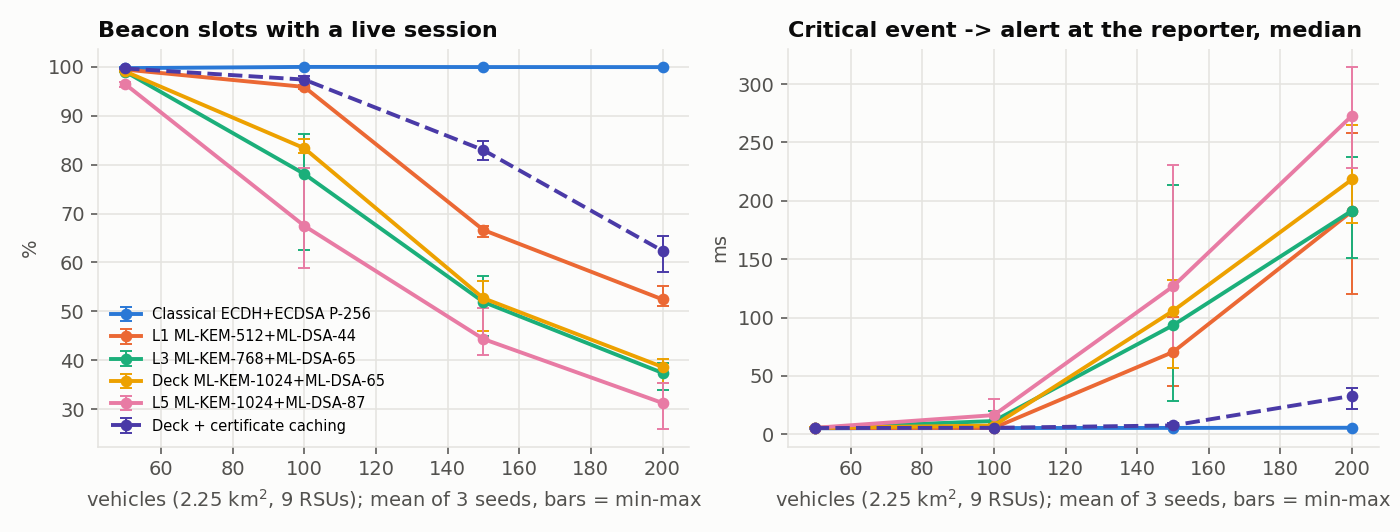
\includegraphics[width=\textwidth]{fig9_ns3_coverage_alert.png}
\caption{Beacon slots with a live session, and the time from a critical event to the alert at the reporting vehicle.}
\label{fig:ns3cov}
\end{figure}

Table~\ref{tab:ns3mid} and Figure~\ref{fig:ns3cov} show the consequence for
safety messaging. A vehicle without a session cannot send authenticated
beacons, so the fraction of beacon slots covered by a session falls with the
handshake success rate. Up to 100 vehicles alerts stay below 20\,ms for every
suite, from \V{ns3-alert-classic-100}\,ms (classical) to
\V{ns3-alert-l5-100}\,ms (L5) median. Beyond that, a saturated channel
delays them too: at 200 vehicles the median is \V{ns3-alert-deck-200}\,ms for
DECK and \V{ns3-alert-deck-cache-200}\,ms with caching, against
\V{ns3-alert-classic-200}\,ms classically.

\subsection{Certificate caching}

\begin{figure}[h]
\centering
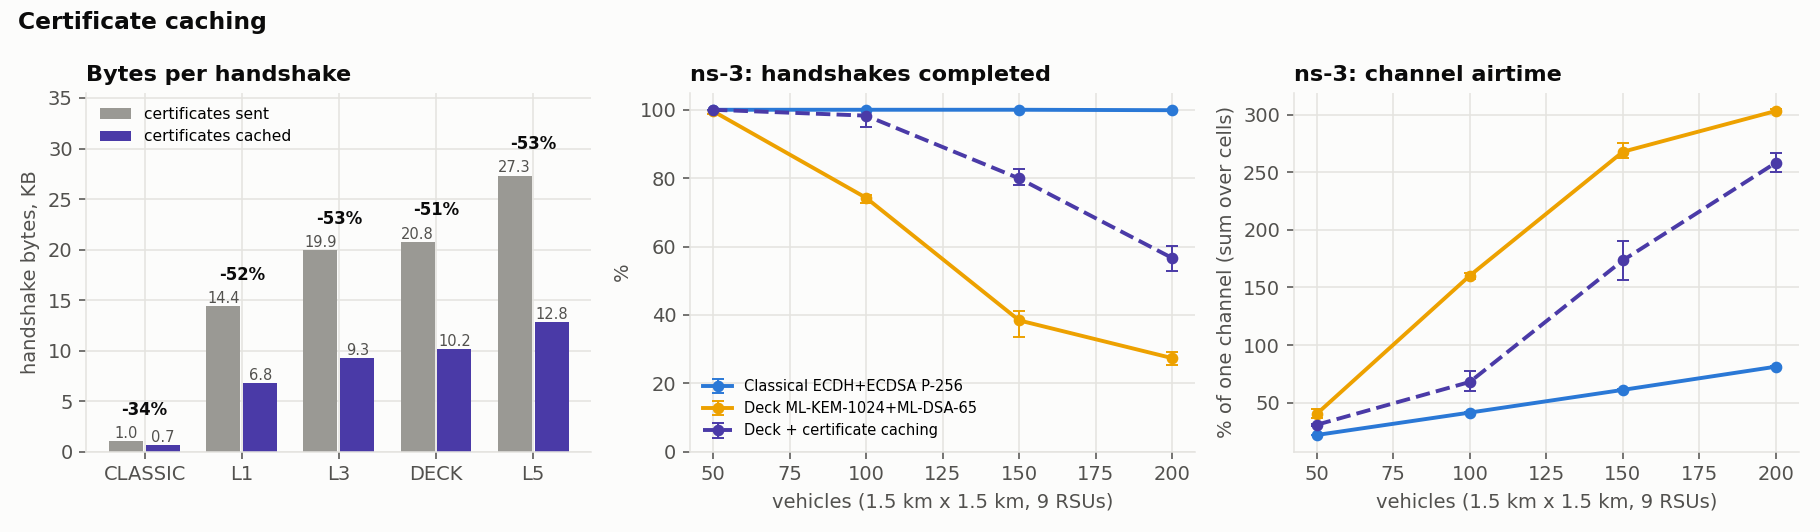
\includegraphics[width=\textwidth]{fig11_cert_cache.png}
\caption{Certificate caching: bytes per handshake for every suite, and its effect on DECK in ns-3.}
\label{fig:cache}
\end{figure}

Caching removes \V{pq-cache-lo}--\V{pq-cache-hi}\,\% of every
post-quantum handshake (Table~\ref{tab:sizes}). In ns-3
(Figure~\ref{fig:cache}), with RSU certificates pre-distributed and vehicle
certificates resolved from the MEC directory, DECK completes
\V{ns3-success-deck-cache-100}\,\% of handshakes at 100 vehicles instead of
\V{ns3-success-deck-100}\,\%, and \V{ns3-success-deck-cache-200}\,\% at 200
instead of \V{ns3-success-deck-200}\,\%; aggregate airtime at 100 vehicles
falls from \V{ns3-airtime-deck-100}\,\% to \V{ns3-airtime-deck-cache-100}\,\%.
Caching does not close the gap to the classical suite: a cached DECK
handshake is still \V{deck-cached-bytes} bytes, about ten times a classical
one, because the ephemeral ML-KEM key, the ciphertext and two ML-DSA
signatures cannot be cached.

\subsection{Variants and mitigations}

\begin{table}[h]
\centering
\caption{Single-seed variants at \V{ns3-mid} vehicles}
\label{tab:variants}
\small
\begin{adjustbox}{max width=\linewidth}
\begin{tabular}{lrrrrr}
\toprule
Scenario (seed 1) & completed \% & p50 ms & coverage \% & alert ms & airtime \% \\
\midrule
DECK, EDCA + backoff (baseline) & 75 & 283 & 82.3 & 7.2 & 157 \\
DECK, neither & 7 & 921 & 40.1 & 432.6 & 339 \\
DECK, EDCA only & 11 & 926 & 44.3 & 382.3 & 330 \\
DECK, backoff only & 77 & 291 & 84.6 & 8.9 & 174 \\
\midrule
DECK + cache (directory) & 100 & 68 & 97.9 & 5.5 & 66 \\
DECK + cache (all warm) & 97 & 66 & 98.5 & 6.0 & 66 \\
L3 + cache (directory) & 100 & 76 & 97.1 & 5.9 & 71 \\
\midrule
DECK, signed beacons & 23 & 704 & 45.9 & 232.9 & 342 \\
Classical, signed beacons & 100 & 9 & 99.9 & 5.4 & 54 \\
\bottomrule
\end{tabular}
\end{adjustbox}
\par\smallskip{\footnotesize Single-seed variants at 100 vehicles. Coverage: beacon slots with a live session. Alert: event $\rightarrow$ alert at the reporter, median. Airtime: summed over all cells.}

\end{table}

\begin{figure}[h]
\centering
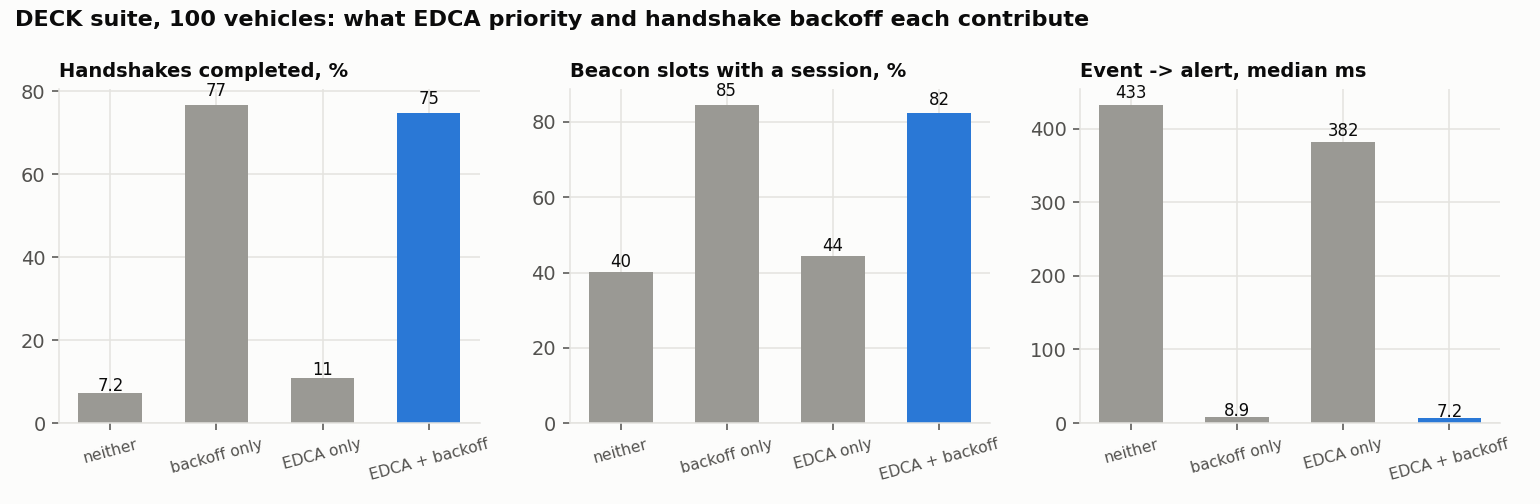
\includegraphics[width=\textwidth]{fig10_ns3_ablation.png}
\caption{Ablation: what EDCA priority and handshake backoff each contribute (DECK, \V{ns3-mid} vehicles).}
\label{fig:ablation}
\end{figure}

Table~\ref{tab:variants} and Figure~\ref{fig:ablation} show four further
results.
\begin{enumerate}
\item \textbf{Exponential backoff prevents congestion collapse.} Without it,
failed handshakes are retried immediately: DECK completes only
\V{var-deck-neither-success}\,\% of handshakes (\V{var-deck-edca-only-success}\,\%
with EDCA alone), and alerts take a median \V{var-deck-neither-alert}\,ms
because they queue behind handshake fragments. With backoff alone DECK
completes \V{var-deck-backoff-only-success}\,\% and alerts take
\V{var-deck-backoff-only-alert}\,ms.
\item \textbf{EDCA priority adds little once backoff is on, at this density.}
With both measures DECK completes \V{var-deck-edca-backoff-baseline-success}\,\%
of handshakes and the alert median is \V{var-deck-edca-backoff-baseline-alert}\,ms,
within single-seed noise of backoff alone. Its value is as a safeguard: it
keeps safety traffic ahead of handshake fragments whenever the queue builds up.
\item \textbf{Signed beacons do not scale with post-quantum signatures.}
Signing every beacon (\V{deck-beacon-signed-frames} frames each) leaves
\V{var-deck-signed-beacons-coverage}\,\% of beacon slots covered, against
\V{var-classical-signed-beacons-coverage}\,\% classically. Session-based AEAD
beacons are the design that scales.
\item \textbf{The implementation still matters in the network.} With
processing times from the pure-Python library, DECK completes
\V{var-deck-pure-python-timings-success}\,\% of handshakes (native:
\V{var-deck-edca-backoff-baseline-success}\,\%) and its median handshake takes
\V{var-deck-pure-python-timings-p50}\,ms instead of
\V{var-deck-edca-backoff-baseline-p50}\,ms.
\end{enumerate}

\section{Consensus}

\begin{table}[h]
\centering
\caption{AGS-PBFT against PBFT}
\label{tab:cons}
\small
\setlength{\tabcolsep}{4pt}
\begin{adjustbox}{max width=\linewidth}
\begin{tabular}{rrrrrrrr}
\toprule
Nodes & $|CN|$ & msgs/req AGS / PBFT & fewer msgs \% & fewer bytes \% & no shadow \% & latency \% & less CPU \% \\
\midrule
8 & 4 & 35 / 128 & 73 & 8 & 41 & +49 & 18 \\
12 & 4 & 47 / 288 & 84 & 23 & 64 & +46 & 25 \\
16 & 7 & 89 / 512 & 83 & 25 & 57 & +41 & 18 \\
20 & 10 & 149 / 800 & 81 & 25 & 53 & +43 & 23 \\
24 & 10 & 161 / 1{,}152 & 86 & 30 & 63 & +58 & 24 \\
\bottomrule
\end{tabular}
\end{adjustbox}
\par\smallskip{\footnotesize Real ML-DSA-65 signatures, 1\,ms links, 20 requests at light load. Percentages are AGS-PBFT relative to PBFT; latency is the median commit latency.}

\end{table}

\begin{figure}[h]
\centering
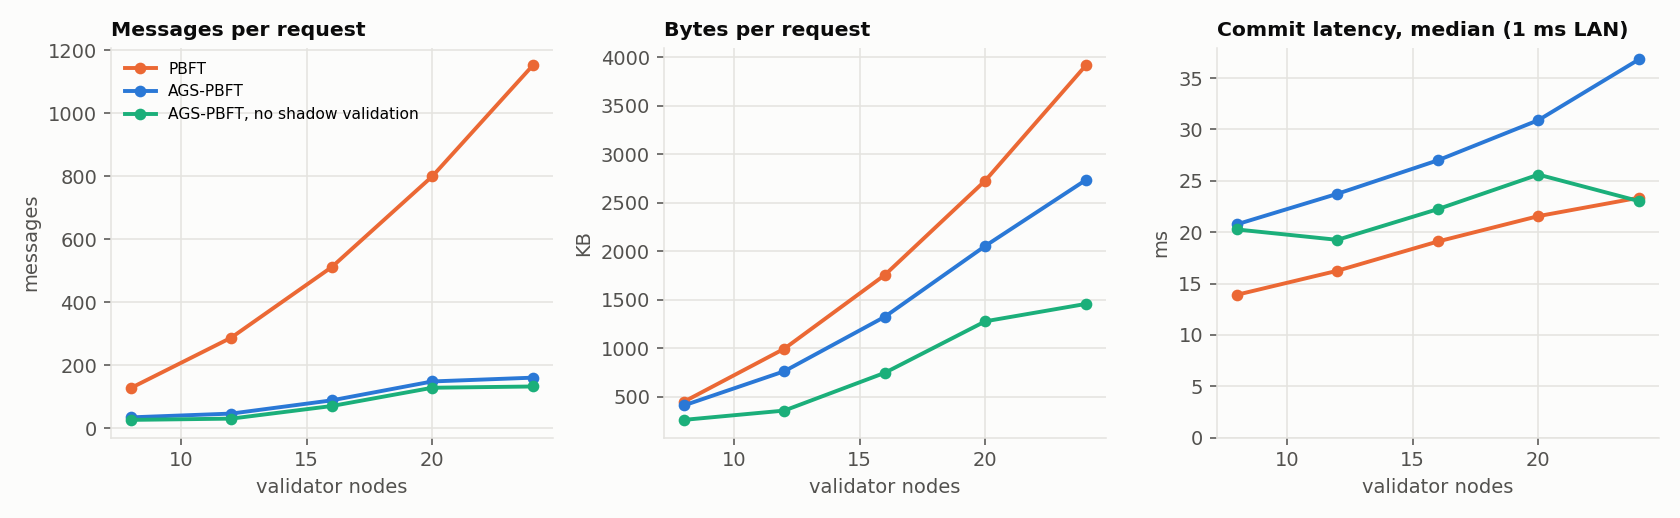
\includegraphics[width=0.9\textwidth]{fig4_consensus_scaling.png}
\caption{Messages, bytes and latency per request against network size.}
\label{fig:cons}
\end{figure}

\textbf{The paper's message saving is real} (Table~\ref{tab:cons},
Figure~\ref{fig:cons}): AGS-PBFT sends \V{cons-msg-8}\,\% fewer messages
than PBFT at 8 nodes and \V{cons-msg-rest-lo}--\V{cons-msg-hi}\,\% fewer at
12--24 nodes, and at light load it uses \V{cons-cpu-lo}--\V{cons-cpu-hi}\,\%
less CPU, because only the $3f+1$ consensus set votes. \textbf{Bytes fall much less}
(\V{cons-byte-lo}--\V{cons-byte-hi}\,\%): every block carries a commit
certificate of $2f+1$ ML-DSA signatures, and with shadow validation (D7) the
candidates' responses as well. Without shadow validation the byte saving is
\V{cons-noshadow-byte-lo}--\V{cons-noshadow-byte-hi}\,\%, but candidates can
then never earn promotion. \textbf{AGS-PBFT is not faster}: replacing PBFT's
parallel all-to-all commit with responses to the leader and a certified block
adds a sequential hop through one node, so commit latency rises by
\V{cons-lat-lo}--\V{cons-lat-hi}\,\%, and under a burst of 60 requests on 16
nodes AGS-PBFT commits \V{tps-ags} requests per second against \V{tps-pbft}
for PBFT, and in that run it used \V{burst-cpu-more}\,\% \emph{more} CPU in
total (\V{burst-cpu-ags}\,s against \V{burst-cpu-pbft}\,s); we have not yet
isolated why the light-load saving reverses under a burst. The paper reports
only the message count.

\begin{table}[h]
\centering
\caption{Fault tolerance}
\label{tab:fault}
\small
\begin{adjustbox}{max width=\linewidth}
\begin{tabular}{lrrrrrr}
\toprule
Byzantine nodes & 0 & 1 & 2 & 3 & 4 & 5 \\
\midrule
Requests committed (\%) & 100 & 100 & 100 & 0 & 0 & 0 \\
Safety held & yes & yes & yes & yes & yes & yes \\
\bottomrule
\end{tabular}
\end{adjustbox}
\par\smallskip{\footnotesize Consensus set 7, f = 2, colluding wrong results, regrouping off.}

\end{table}

\begin{table}[h]
\centering
\caption{Recovery after a leader crash}
\label{tab:vc}
\small
\begin{adjustbox}{max width=\linewidth}
\begin{tabular}{lrr}
\toprule
View-change timeout & AGS-PBFT & PBFT \\
\midrule
0.5 s & 1.21 s & 1.19 s \\
1.0 s & 2.22 s & 2.17 s \\
2.0 s & 4.72 s & 4.68 s \\
\bottomrule
\end{tabular}
\end{adjustbox}
\par\smallskip{\footnotesize Time from the leader's crash to the first commit in the new view (8 nodes).}

\end{table}

Table~\ref{tab:fault} shows PBFT's liveness bound: up to $f$ colluding
Byzantine nodes nothing changes, and beyond $f$ the honest nodes can no longer
form a $2f+1$ quorum, so progress stops. No false result was committed in any
run, but this experiment keeps the leader honest, and an honest leader never
certifies a result that differs from its own. With 5 colluders in a set of 7
the colluders could form a quorum of 5 on their own, so a Byzantine
\emph{leader} beyond $f$ could commit a false result, exactly as PBFT theory
predicts. Recovery after a leader crash (Table~\ref{tab:vc}) takes about
2.2--2.4 times the view-change timeout, because the client's retransmission
timeout and the backups' view-change timeout run one after the other.

\begin{figure}[h]
\centering
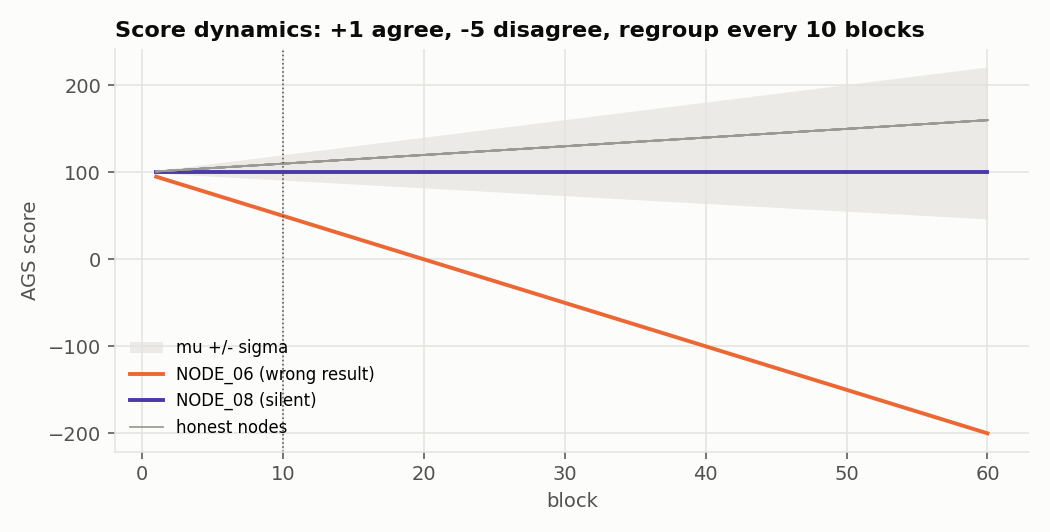
\includegraphics[width=0.9\textwidth]{fig5_score_dynamics.png}
\caption{Score dynamics with one wrong-result node and one silent node (16 nodes, regroup every 10 blocks).}
\label{fig:scores}
\end{figure}

Figure~\ref{fig:scores} shows a weakness of the paper's $\mu \pm \sigma$
rule. The wrong-result node loses 5 points per block and is demoted at the
first regroup. The silent node keeps its score of 100 while honest nodes
climb, but the wrong-result node's extreme score inflates $\sigma$ so much
that $\mu - \sigma$ stays below 100, and the silent node is never demoted.
Without the outlier it is demoted (a regression test checks both cases). A
robust statistic, such as the median and the median absolute deviation, would
not be distorted by one extreme node.

\section{Security}

\begin{table}[h]
\centering
\caption{Attacks run against the implementation}
\label{tab:attacks}
\scriptsize
\begin{adjustbox}{max width=\linewidth}
\begin{tabular}{p{5.4cm}cp{7.2cm}}
\toprule
Attack & Rejected & Mechanism \\
\midrule
record tampering (1 bit flipped) & yes & AES-256-GCM tag check fails \\
record replay & yes & counter already seen in the 64-record window \\
GCM nonce reuse with Finished & yes & data counters start at 1; 0 is Finished only \\
ClientHello replay & yes & nonce already in the server's replay cache \\
stale ClientHello (timestamp -300 s) & yes & outside the 30 s freshness window \\
client impersonation with stolen certificate & yes & client signature over the transcript fails (deck design had no client signature) \\
RSU impersonation with stolen certificate & yes & server signature over transcript + pk\_kem fails \\
certificate from a rogue TA & yes & certificate signature does not verify under pk\_TA \\
revoked credential & yes & certificate serial on the signed CRL \\
cache: claim another vehicle's cached certificate & yes & client signature checked with the referenced certificate's key \\
cache: revoked certificate still in the cache & yes & cached certificates are re-verified against the current CRL \\
vehicle posing as an RSU & yes & role is bound into the certificate \\
MITM substitutes the ephemeral ML-KEM key & yes & server signature covers pk\_kem \\
MITM substitutes the KEM ciphertext & yes & client signature covers c \\
downgrade to classical suite & yes & suite must match and is inside both signatures \\
tampered Finished & yes & key confirmation under transcript-bound keys fails \\
forward secrecy: ephemeral key retained & yes & ephemeral ML-KEM key per session, erased after decapsulation \\
consensus vote from a non-member & yes & sender has no certificate in the directory \\
consensus vote spoofing another member & yes & ML-DSA signature does not verify \\
tampered block (result changed) & yes & leader signature and commit certificate \\
ledger history rewrite & yes & Pr\_B\_Hash link broken \\
\bottomrule
\end{tabular}
\end{adjustbox}

\end{table}

All \V{attacks-total} attacks in Table~\ref{tab:attacks} were rejected. Client
impersonation with a copied certificate would succeed against the Review~1
design, which had no client signature (F2).

\section{Answers to the research questions}

\begin{enumerate}
\item \textbf{Can the framework be implemented with the standardised
algorithms?} Yes, after the corrections D1--D5 and F1--F7 and the design
decisions D6--D9; the result runs as a distributed system and withstands the
tested attacks.
\item \textbf{Does post-quantum protection fit the 100\,ms budget?} Per
message, yes, at every security level: \V{deck-beacon-aead}\,ms per beacon
inside a session, or \V{deck-beacon-signed}\,ms for a natively signed beacon.
A full handshake costs about \V{deck-hs-ms}\,ms of computation natively.
\item \textbf{How does the channel behave as density grows?} The handshake
is the problem: at 100 vehicles DECK completes \V{ns3-success-deck-100}\,\% of
handshakes against \V{ns3-success-classic-100}\,\% classically. Certificate
caching and exponential backoff recover much of the loss; a smaller KEM (L3
instead of DECK) costs nothing in security, since DECK's strength is set by
its category-3 signature.
\item \textbf{Does AGS-PBFT beat PBFT?} On messages, yes, and on CPU at
light load; on bytes, modestly; on latency, burst throughput and CPU under a
burst, no. It never sits on the safety path.
\end{enumerate}

\chapter{Conclusion and Future Work}
\label{ch:conc}

\section{Conclusion}

We built a complete post-quantum security framework for connected vehicles,
from registration with a Trusted Authority through a mutually authenticated
ML-KEM/ML-DSA handshake and encrypted records to AGS-PBFT consensus over a
verifiable ledger, and ran it as a distributed system, in an 802.11p
simulation with mobility, and under attack. Implementing the base paper
exposed defects that prevent it from working as published, the most serious
being a consensus layer that signs with a KEM; implementing our own Review~1
design exposed the lack of client authentication. Both were corrected and the
corrections tested.

The measurements answer the project's question. Post-quantum cryptography
fits the vehicular latency budget per message, at every NIST security level,
once it is implemented natively: a beacon inside a session is a
\V{deck-beacon-aead-bytes}-byte AES-GCM record whatever the suite, and a full
handshake takes about \V{deck-hs-ms}\,ms of computation. The binding
constraint is size. A post-quantum handshake is about twenty times larger
than a classical one, and on a shared 6\,Mb/s channel that is what fails as
density grows: at 100 vehicles in our scenario DECK completes
\V{ns3-success-deck-100}\,\% of handshakes, against
\V{ns3-success-classic-100}\,\% classically. Protocol design recovers much of
the loss. Certificate caching halves the handshake and raises completion to
\V{ns3-success-deck-cache-100}\,\%, and exponential backoff after a failed
handshake prevents congestion collapse. Safety warnings do not wait
for consensus at all, and AGS-PBFT saves messages, and CPU at light load, but not time.

\section{Limitations}

\begin{itemize}
\item \textbf{One machine.} The distributed system runs on localhost, so its
latencies include TCP over loopback, not radio. Radio effects come only from
ns-3.
\item \textbf{ns-3 replays measured costs.} The simulation uses measured
message sizes and processing-time distributions rather than executing the
cryptography.
\item \textbf{No WAVE module.} The ns-3 Python package provides the 802.11p
PHY and MAC but no WAVE/OCB module, so the ad-hoc MAC is used. Ad-hoc mode
also has no association, so behaviour is close.
\item \textbf{Certificate caching relies on infrastructure we model.} The
edge directory is the TA registry in the distributed system and one backhaul
round trip in ns-3. A vehicle's first handshake still sends its certificate in
full.
\item \textbf{Linkability.} Certificates and certificate references identify a
vehicle across handshakes; pseudonym certificates would be needed for
location privacy.
\item \textbf{V2V through RSUs is not end-to-end.} Relaying RSUs see the
plaintext, as in the original design.
\item \textbf{No formal verification} of the handshake.
\end{itemize}

\section{Future work}

\begin{itemize}
\item \textbf{Smaller handshakes.} KEM-based authentication in the style of
KEMTLS, which replaces the server's signature with a KEM, or certificates
signed with a scheme that has smaller signatures, would attack the remaining
size directly.
\item \textbf{Robust regrouping.} Replace AGS-PBFT's $\mu \pm \sigma$ rule
with the median and median absolute deviation, so that one outlier cannot
shield a silent node.
\item \textbf{Formal analysis} of the handshake, including certificate
caching, with a protocol verifier such as ProVerif or Tamarin.
\item \textbf{Pseudonymous certificates} compatible with caching.
\item \textbf{Realistic mobility} from a traffic simulator on a real road
network, and evaluation on vehicular hardware.
\end{itemize}


\begin{thebibliography}{99}
\addcontentsline{toc}{chapter}{References}

\bibitem{base} A.~M. Aslam, A.~Bhardwaj and R.~Chaudhary, ``Quantum-resilient blockchain-enabled secure communication framework for connected autonomous vehicles using post-quantum cryptography,'' \emph{Vehicular Communications}, vol.~52, art.~100880, 2025, doi:10.1016/j.vehcom.2025.100880.

% TODO (team): add the article title from the paper.
\bibitem{olushola} A.~Olushola and S.~P. Meenakshi, ``[article title],'' \emph{Frontiers in Physics}, vol.~13, art.~1723966, 2025.

\bibitem{fips203} National Institute of Standards and Technology, \emph{Module-Lattice-Based Key-Encapsulation Mechanism Standard}, FIPS~203, Aug.~2024.

\bibitem{fips204} National Institute of Standards and Technology, \emph{Module-Lattice-Based Digital Signature Standard}, FIPS~204, Aug.~2024.

\bibitem{nistir8547} National Institute of Standards and Technology, \emph{Transition to Post-Quantum Cryptography Standards}, NIST IR~8547 (initial public draft), Nov.~2024.

\bibitem{shor} P.~W. Shor, ``Polynomial-time algorithms for prime factorization and discrete logarithms on a quantum computer,'' \emph{SIAM Journal on Computing}, vol.~26, no.~5, pp.~1484--1509, 1997.

\bibitem{grover} L.~K. Grover, ``A fast quantum mechanical algorithm for database search,'' in \emph{Proc. 28th ACM Symposium on Theory of Computing}, 1996, pp.~212--219.

\bibitem{mosca} M.~Mosca, ``Cybersecurity in an era with quantum computers: will we be ready?'' \emph{IEEE Security \& Privacy}, vol.~16, no.~5, pp.~38--41, 2018.

\bibitem{kyber} J.~Bos, L.~Ducas, E.~Kiltz, T.~Lepoint, V.~Lyubashevsky, J.~M. Schanck, P.~Schwabe, G.~Seiler and D.~Stehl\'e, ``CRYSTALS-Kyber: a CCA-secure module-lattice-based KEM,'' in \emph{Proc. IEEE European Symposium on Security and Privacy}, 2018, pp.~353--367.

\bibitem{dilithium} L.~Ducas, E.~Kiltz, T.~Lepoint, V.~Lyubashevsky, P.~Schwabe, G.~Seiler and D.~Stehl\'e, ``CRYSTALS-Dilithium: a lattice-based digital signature scheme,'' \emph{IACR Transactions on Cryptographic Hardware and Embedded Systems}, vol.~2018, no.~1, pp.~238--268, 2018.

\bibitem{regev} O.~Regev, ``On lattices, learning with errors, random linear codes, and cryptography,'' \emph{Journal of the ACM}, vol.~56, no.~6, art.~34, 2009.

\bibitem{langlois} A.~Langlois and D.~Stehl\'e, ``Worst-case to average-case reductions for module lattices,'' \emph{Designs, Codes and Cryptography}, vol.~75, no.~3, pp.~565--599, 2015.

\bibitem{fo} E.~Fujisaki and T.~Okamoto, ``Secure integration of asymmetric and symmetric encryption schemes,'' in \emph{Advances in Cryptology -- CRYPTO '99}, LNCS 1666, 1999, pp.~537--554.

\bibitem{pbft} M.~Castro and B.~Liskov, ``Practical Byzantine fault tolerance,'' in \emph{Proc. 3rd USENIX Symposium on Operating Systems Design and Implementation (OSDI)}, 1999, pp.~173--186.

\bibitem{fabric} E.~Androulaki et~al., ``Hyperledger Fabric: a distributed operating system for permissioned blockchains,'' in \emph{Proc. 13th EuroSys Conference}, 2018, art.~30.

\bibitem{ieee16092} \emph{IEEE Standard for Wireless Access in Vehicular Environments---Security Services for Application and Management Messages}, IEEE Std 1609.2-2022.

\bibitem{ieee80211p} \emph{IEEE Standard for Information Technology---Part 11: Wireless LAN MAC and PHY Specifications, Amendment 6: Wireless Access in Vehicular Environments}, IEEE Std 802.11p-2010.

\bibitem{torrent} M.~Torrent-Moreno, D.~Jiang and H.~Hartenstein, ``Broadcast reception rates and effects of priority access in 802.11-based vehicular ad-hoc networks,'' in \emph{Proc. 1st ACM International Workshop on Vehicular Ad Hoc Networks (VANET)}, 2004, pp.~10--18.

\bibitem{ns3} G.~F. Riley and T.~R. Henderson, ``The ns-3 network simulator,'' in \emph{Modeling and Tools for Network Simulation}, Springer, 2010, pp.~15--34.

\bibitem{tls13} E.~Rescorla, \emph{The Transport Layer Security (TLS) Protocol Version 1.3}, RFC~8446, 2018.

\bibitem{rfc7924} S.~Santesson and H.~Tschofenig, \emph{Transport Layer Security (TLS) Cached Information Extension}, RFC~7924, 2016.

\bibitem{hpke} R.~Barnes, K.~Bhargavan, B.~Lipp and C.~Wood, \emph{Hybrid Public Key Encryption}, RFC~9180, 2022.

\bibitem{hkdf} H.~Krawczyk and P.~Eronen, \emph{HMAC-based Extract-and-Expand Key Derivation Function (HKDF)}, RFC~5869, 2010.

\bibitem{gcm} M.~Dworkin, \emph{Recommendation for Block Cipher Modes of Operation: Galois/Counter Mode (GCM) and GMAC}, NIST SP~800-38D, 2007.

\bibitem{esp} S.~Kent, \emph{IP Encapsulating Security Payload (ESP)}, RFC~4303, 2005.

\end{thebibliography}


\appendix
\chapter{Running the System}
\label{app:run}

\section{Installation}

\begin{lstlisting}
python -m venv .venv
.venv\Scripts\activate              # Linux/macOS: source .venv/bin/activate
pip install -r requirements.txt     # cryptography>=47, kyber-py, ...
\end{lstlisting}

The ns-3 experiments need Linux or WSL2:
\begin{lstlisting}
pip install -r requirements.txt -r requirements-ns3.txt
\end{lstlisting}

\section{Commands}

\begin{table}[h]
\centering
\caption{Commands}
\small
\begin{tabular}{@{}p{8.6cm}p{5.4cm}@{}}
\toprule
Command & Purpose \\
\midrule
\code{python scripts/demo\_protocol.py} & the protocol step by step, with attacks \\
\code{python scripts/run\_network.py} & the 19-process distributed system \\
\code{python -m pytest} & the 55 tests \\
\code{python scripts/run\_evaluation.py} & benchmarks, attacks, consensus, figures \\
\code{python scripts/run\_ns3\_sweeps.py} & ns-3 density sweep and variants \\
\code{python scripts/run\_ns3\_sweeps.py --seeds 2 3} & extra seeds \\
\code{python scripts/make\_viewer.py} & the replay viewer (\code{results/viewer.html}) \\
\code{python scripts/make\_tables.py} & this report's tables and numbers \\
\bottomrule
\end{tabular}
\end{table}

\section{Replay viewer}

\begin{figure}[h]
\centering
\IfFileExists{../results/viewer_screenshot.png}{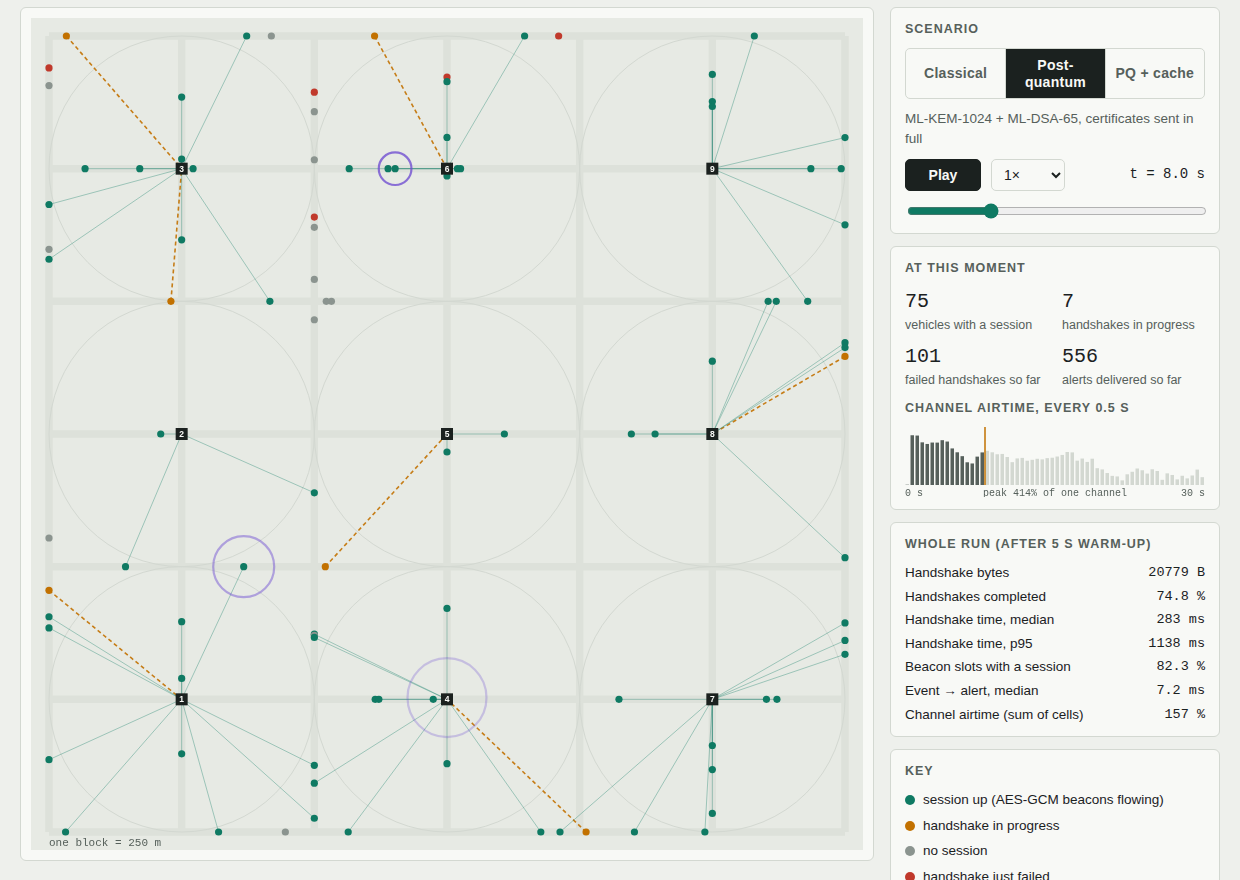
\includegraphics[width=\textwidth]{viewer_screenshot.png}}{\fbox{viewer screenshot}}
\caption{The replay viewer: vehicles (dots) on the 1.5\,km grid, RSUs (squares), handshakes in progress (dashed) and sessions (solid), with the channel airtime over time. The same run can be switched between the classical suite, DECK and DECK with certificate caching.}
\label{fig:viewer}
\end{figure}


\end{document}
